\documentclass[twoside]{article}

\usepackage[accepted]{aistats2025}




\usepackage{wrapfig}

% If you use the following package, be sure to comment out \usepackate{xcolor}

\usepackage{multirow,mathtools } \usepackage{algorithm,algpseudocode}

% Very useful for various special symbols
\usepackage{pifont}
% For \rowcolor
\usepackage{color, colortbl}

\usepackage{blindtext}
\usepackage{lipsum}

\usepackage{multirow}
\usepackage{graphicx}
\usepackage{listings}

\usepackage{bbm}
\usepackage{dsfont}

\usepackage[most]{tcolorbox}

\newcommand{\JH}[1]{\textcolor{blue}{JH: #1}}
\newcommand{\SL}[1]{\textcolor{purple}{SL: #1}}
\newcommand{\JC}[1]{\textcolor{cyan}{JC: #1}}
\newcommand{\SM}[1]{\textcolor{red}{SM: #1}}
\newcommand{\CF}[1]{\textcolor{orange}{CF: #1}}
\newcommand{\RZ}[1]{\textcolor{red}{RZ: #1}}
\newcommand{\LL}[1]{\textcolor{red}{LL: #1}}
\newcommand{\YY}[1]{\textcolor{red}{YY: #1}}

%%%%% NEW MATH DEFINITIONS %%%%%

\usepackage{amsmath,amsfonts,bm}
\usepackage{derivative}
% Mark sections of captions for referring to divisions of figures
\newcommand{\figleft}{{\em (Left)}}
\newcommand{\figcenter}{{\em (Center)}}
\newcommand{\figright}{{\em (Right)}}
\newcommand{\figtop}{{\em (Top)}}
\newcommand{\figbottom}{{\em (Bottom)}}
\newcommand{\captiona}{{\em (a)}}
\newcommand{\captionb}{{\em (b)}}
\newcommand{\captionc}{{\em (c)}}
\newcommand{\captiond}{{\em (d)}}

% Highlight a newly defined term
\newcommand{\newterm}[1]{{\bf #1}}

% Derivative d 
\newcommand{\deriv}{{\mathrm{d}}}

% Figure reference, lower-case.
\def\figref#1{figure~\ref{#1}}
% Figure reference, capital. For start of sentence
\def\Figref#1{Figure~\ref{#1}}
\def\twofigref#1#2{figures \ref{#1} and \ref{#2}}
\def\quadfigref#1#2#3#4{figures \ref{#1}, \ref{#2}, \ref{#3} and \ref{#4}}
% Section reference, lower-case.
\def\secref#1{section~\ref{#1}}
% Section reference, capital.
\def\Secref#1{Section~\ref{#1}}
% Reference to two sections.
\def\twosecrefs#1#2{sections \ref{#1} and \ref{#2}}
% Reference to three sections.
\def\secrefs#1#2#3{sections \ref{#1}, \ref{#2} and \ref{#3}}
% Reference to an equation, lower-case.
\def\eqref#1{equation~\ref{#1}}
% Reference to an equation, upper case
\def\Eqref#1{Equation~\ref{#1}}
% A raw reference to an equation---avoid using if possible
\def\plaineqref#1{\ref{#1}}
% Reference to a chapter, lower-case.
\def\chapref#1{chapter~\ref{#1}}
% Reference to an equation, upper case.
\def\Chapref#1{Chapter~\ref{#1}}
% Reference to a range of chapters
\def\rangechapref#1#2{chapters\ref{#1}--\ref{#2}}
% Reference to an algorithm, lower-case.
\def\algref#1{algorithm~\ref{#1}}
% Reference to an algorithm, upper case.
\def\Algref#1{Algorithm~\ref{#1}}
\def\twoalgref#1#2{algorithms \ref{#1} and \ref{#2}}
\def\Twoalgref#1#2{Algorithms \ref{#1} and \ref{#2}}
% Reference to a part, lower case
\def\partref#1{part~\ref{#1}}
% Reference to a part, upper case
\def\Partref#1{Part~\ref{#1}}
\def\twopartref#1#2{parts \ref{#1} and \ref{#2}}

\def\ceil#1{\lceil #1 \rceil}
\def\floor#1{\lfloor #1 \rfloor}
\def\1{\bm{1}}
\newcommand{\train}{\mathcal{D}}
\newcommand{\valid}{\mathcal{D_{\mathrm{valid}}}}
\newcommand{\test}{\mathcal{D_{\mathrm{test}}}}

\def\eps{{\epsilon}}


% Random variables
\def\reta{{\textnormal{$\eta$}}}
\def\ra{{\textnormal{a}}}
\def\rb{{\textnormal{b}}}
\def\rc{{\textnormal{c}}}
\def\rd{{\textnormal{d}}}
\def\re{{\textnormal{e}}}
\def\rf{{\textnormal{f}}}
\def\rg{{\textnormal{g}}}
\def\rh{{\textnormal{h}}}
\def\ri{{\textnormal{i}}}
\def\rj{{\textnormal{j}}}
\def\rk{{\textnormal{k}}}
\def\rl{{\textnormal{l}}}
% rm is already a command, just don't name any random variables m
\def\rn{{\textnormal{n}}}
\def\ro{{\textnormal{o}}}
\def\rp{{\textnormal{p}}}
\def\rq{{\textnormal{q}}}
\def\rr{{\textnormal{r}}}
\def\rs{{\textnormal{s}}}
\def\rt{{\textnormal{t}}}
\def\ru{{\textnormal{u}}}
\def\rv{{\textnormal{v}}}
\def\rw{{\textnormal{w}}}
\def\rx{{\textnormal{x}}}
\def\ry{{\textnormal{y}}}
\def\rz{{\textnormal{z}}}

% Random vectors
\def\rvepsilon{{\mathbf{\epsilon}}}
\def\rvphi{{\mathbf{\phi}}}
\def\rvtheta{{\mathbf{\theta}}}
\def\rva{{\mathbf{a}}}
\def\rvb{{\mathbf{b}}}
\def\rvc{{\mathbf{c}}}
\def\rvd{{\mathbf{d}}}
\def\rve{{\mathbf{e}}}
\def\rvf{{\mathbf{f}}}
\def\rvg{{\mathbf{g}}}
\def\rvh{{\mathbf{h}}}
\def\rvu{{\mathbf{i}}}
\def\rvj{{\mathbf{j}}}
\def\rvk{{\mathbf{k}}}
\def\rvl{{\mathbf{l}}}
\def\rvm{{\mathbf{m}}}
\def\rvn{{\mathbf{n}}}
\def\rvo{{\mathbf{o}}}
\def\rvp{{\mathbf{p}}}
\def\rvq{{\mathbf{q}}}
\def\rvr{{\mathbf{r}}}
\def\rvs{{\mathbf{s}}}
\def\rvt{{\mathbf{t}}}
\def\rvu{{\mathbf{u}}}
\def\rvv{{\mathbf{v}}}
\def\rvw{{\mathbf{w}}}
\def\rvx{{\mathbf{x}}}
\def\rvy{{\mathbf{y}}}
\def\rvz{{\mathbf{z}}}

% Elements of random vectors
\def\erva{{\textnormal{a}}}
\def\ervb{{\textnormal{b}}}
\def\ervc{{\textnormal{c}}}
\def\ervd{{\textnormal{d}}}
\def\erve{{\textnormal{e}}}
\def\ervf{{\textnormal{f}}}
\def\ervg{{\textnormal{g}}}
\def\ervh{{\textnormal{h}}}
\def\ervi{{\textnormal{i}}}
\def\ervj{{\textnormal{j}}}
\def\ervk{{\textnormal{k}}}
\def\ervl{{\textnormal{l}}}
\def\ervm{{\textnormal{m}}}
\def\ervn{{\textnormal{n}}}
\def\ervo{{\textnormal{o}}}
\def\ervp{{\textnormal{p}}}
\def\ervq{{\textnormal{q}}}
\def\ervr{{\textnormal{r}}}
\def\ervs{{\textnormal{s}}}
\def\ervt{{\textnormal{t}}}
\def\ervu{{\textnormal{u}}}
\def\ervv{{\textnormal{v}}}
\def\ervw{{\textnormal{w}}}
\def\ervx{{\textnormal{x}}}
\def\ervy{{\textnormal{y}}}
\def\ervz{{\textnormal{z}}}

% Random matrices
\def\rmA{{\mathbf{A}}}
\def\rmB{{\mathbf{B}}}
\def\rmC{{\mathbf{C}}}
\def\rmD{{\mathbf{D}}}
\def\rmE{{\mathbf{E}}}
\def\rmF{{\mathbf{F}}}
\def\rmG{{\mathbf{G}}}
\def\rmH{{\mathbf{H}}}
\def\rmI{{\mathbf{I}}}
\def\rmJ{{\mathbf{J}}}
\def\rmK{{\mathbf{K}}}
\def\rmL{{\mathbf{L}}}
\def\rmM{{\mathbf{M}}}
\def\rmN{{\mathbf{N}}}
\def\rmO{{\mathbf{O}}}
\def\rmP{{\mathbf{P}}}
\def\rmQ{{\mathbf{Q}}}
\def\rmR{{\mathbf{R}}}
\def\rmS{{\mathbf{S}}}
\def\rmT{{\mathbf{T}}}
\def\rmU{{\mathbf{U}}}
\def\rmV{{\mathbf{V}}}
\def\rmW{{\mathbf{W}}}
\def\rmX{{\mathbf{X}}}
\def\rmY{{\mathbf{Y}}}
\def\rmZ{{\mathbf{Z}}}

% Elements of random matrices
\def\ermA{{\textnormal{A}}}
\def\ermB{{\textnormal{B}}}
\def\ermC{{\textnormal{C}}}
\def\ermD{{\textnormal{D}}}
\def\ermE{{\textnormal{E}}}
\def\ermF{{\textnormal{F}}}
\def\ermG{{\textnormal{G}}}
\def\ermH{{\textnormal{H}}}
\def\ermI{{\textnormal{I}}}
\def\ermJ{{\textnormal{J}}}
\def\ermK{{\textnormal{K}}}
\def\ermL{{\textnormal{L}}}
\def\ermM{{\textnormal{M}}}
\def\ermN{{\textnormal{N}}}
\def\ermO{{\textnormal{O}}}
\def\ermP{{\textnormal{P}}}
\def\ermQ{{\textnormal{Q}}}
\def\ermR{{\textnormal{R}}}
\def\ermS{{\textnormal{S}}}
\def\ermT{{\textnormal{T}}}
\def\ermU{{\textnormal{U}}}
\def\ermV{{\textnormal{V}}}
\def\ermW{{\textnormal{W}}}
\def\ermX{{\textnormal{X}}}
\def\ermY{{\textnormal{Y}}}
\def\ermZ{{\textnormal{Z}}}

% Vectors
\def\vzero{{\bm{0}}}
\def\vone{{\bm{1}}}
\def\vmu{{\bm{\mu}}}
\def\vtheta{{\bm{\theta}}}
\def\vphi{{\bm{\phi}}}
\def\va{{\bm{a}}}
\def\vb{{\bm{b}}}
\def\vc{{\bm{c}}}
\def\vd{{\bm{d}}}
\def\ve{{\bm{e}}}
\def\vf{{\bm{f}}}
\def\vg{{\bm{g}}}
\def\vh{{\bm{h}}}
\def\vi{{\bm{i}}}
\def\vj{{\bm{j}}}
\def\vk{{\bm{k}}}
\def\vl{{\bm{l}}}
\def\vm{{\bm{m}}}
\def\vn{{\bm{n}}}
\def\vo{{\bm{o}}}
\def\vp{{\bm{p}}}
\def\vq{{\bm{q}}}
\def\vr{{\bm{r}}}
\def\vs{{\bm{s}}}
\def\vt{{\bm{t}}}
\def\vu{{\bm{u}}}
\def\vv{{\bm{v}}}
\def\vw{{\bm{w}}}
\def\vx{{\bm{x}}}
\def\vy{{\bm{y}}}
\def\vz{{\bm{z}}}

% Elements of vectors
\def\evalpha{{\alpha}}
\def\evbeta{{\beta}}
\def\evepsilon{{\epsilon}}
\def\evlambda{{\lambda}}
\def\evomega{{\omega}}
\def\evmu{{\mu}}
\def\evpsi{{\psi}}
\def\evsigma{{\sigma}}
\def\evtheta{{\theta}}
\def\eva{{a}}
\def\evb{{b}}
\def\evc{{c}}
\def\evd{{d}}
\def\eve{{e}}
\def\evf{{f}}
\def\evg{{g}}
\def\evh{{h}}
\def\evi{{i}}
\def\evj{{j}}
\def\evk{{k}}
\def\evl{{l}}
\def\evm{{m}}
\def\evn{{n}}
\def\evo{{o}}
\def\evp{{p}}
\def\evq{{q}}
\def\evr{{r}}
\def\evs{{s}}
\def\evt{{t}}
\def\evu{{u}}
\def\evv{{v}}
\def\evw{{w}}
\def\evx{{x}}
\def\evy{{y}}
\def\evz{{z}}

% Matrix
\def\mA{{\bm{A}}}
\def\mB{{\bm{B}}}
\def\mC{{\bm{C}}}
\def\mD{{\bm{D}}}
\def\mE{{\bm{E}}}
\def\mF{{\bm{F}}}
\def\mG{{\bm{G}}}
\def\mH{{\bm{H}}}
\def\mI{{\bm{I}}}
\def\mJ{{\bm{J}}}
\def\mK{{\bm{K}}}
\def\mL{{\bm{L}}}
\def\mM{{\bm{M}}}
\def\mN{{\bm{N}}}
\def\mO{{\bm{O}}}
\def\mP{{\bm{P}}}
\def\mQ{{\bm{Q}}}
\def\mR{{\bm{R}}}
\def\mS{{\bm{S}}}
\def\mT{{\bm{T}}}
\def\mU{{\bm{U}}}
\def\mV{{\bm{V}}}
\def\mW{{\bm{W}}}
\def\mX{{\bm{X}}}
\def\mY{{\bm{Y}}}
\def\mZ{{\bm{Z}}}
\def\mBeta{{\bm{\beta}}}
\def\mPhi{{\bm{\Phi}}}
\def\mLambda{{\bm{\Lambda}}}
\def\mSigma{{\bm{\Sigma}}}

% Tensor
\DeclareMathAlphabet{\mathsfit}{\encodingdefault}{\sfdefault}{m}{sl}
\SetMathAlphabet{\mathsfit}{bold}{\encodingdefault}{\sfdefault}{bx}{n}
\newcommand{\tens}[1]{\bm{\mathsfit{#1}}}
\def\tA{{\tens{A}}}
\def\tB{{\tens{B}}}
\def\tC{{\tens{C}}}
\def\tD{{\tens{D}}}
\def\tE{{\tens{E}}}
\def\tF{{\tens{F}}}
\def\tG{{\tens{G}}}
\def\tH{{\tens{H}}}
\def\tI{{\tens{I}}}
\def\tJ{{\tens{J}}}
\def\tK{{\tens{K}}}
\def\tL{{\tens{L}}}
\def\tM{{\tens{M}}}
\def\tN{{\tens{N}}}
\def\tO{{\tens{O}}}
\def\tP{{\tens{P}}}
\def\tQ{{\tens{Q}}}
\def\tR{{\tens{R}}}
\def\tS{{\tens{S}}}
\def\tT{{\tens{T}}}
\def\tU{{\tens{U}}}
\def\tV{{\tens{V}}}
\def\tW{{\tens{W}}}
\def\tX{{\tens{X}}}
\def\tY{{\tens{Y}}}
\def\tZ{{\tens{Z}}}


% Graph
\def\gA{{\mathcal{A}}}
\def\gB{{\mathcal{B}}}
\def\gC{{\mathcal{C}}}
\def\gD{{\mathcal{D}}}
\def\gE{{\mathcal{E}}}
\def\gF{{\mathcal{F}}}
\def\gG{{\mathcal{G}}}
\def\gH{{\mathcal{H}}}
\def\gI{{\mathcal{I}}}
\def\gJ{{\mathcal{J}}}
\def\gK{{\mathcal{K}}}
\def\gL{{\mathcal{L}}}
\def\gM{{\mathcal{M}}}
\def\gN{{\mathcal{N}}}
\def\gO{{\mathcal{O}}}
\def\gP{{\mathcal{P}}}
\def\gQ{{\mathcal{Q}}}
\def\gR{{\mathcal{R}}}
\def\gS{{\mathcal{S}}}
\def\gT{{\mathcal{T}}}
\def\gU{{\mathcal{U}}}
\def\gV{{\mathcal{V}}}
\def\gW{{\mathcal{W}}}
\def\gX{{\mathcal{X}}}
\def\gY{{\mathcal{Y}}}
\def\gZ{{\mathcal{Z}}}

% Sets
\def\sA{{\mathbb{A}}}
\def\sB{{\mathbb{B}}}
\def\sC{{\mathbb{C}}}
\def\sD{{\mathbb{D}}}
% Don't use a set called E, because this would be the same as our symbol
% for expectation.
\def\sF{{\mathbb{F}}}
\def\sG{{\mathbb{G}}}
\def\sH{{\mathbb{H}}}
\def\sI{{\mathbb{I}}}
\def\sJ{{\mathbb{J}}}
\def\sK{{\mathbb{K}}}
\def\sL{{\mathbb{L}}}
\def\sM{{\mathbb{M}}}
\def\sN{{\mathbb{N}}}
\def\sO{{\mathbb{O}}}
\def\sP{{\mathbb{P}}}
\def\sQ{{\mathbb{Q}}}
\def\sR{{\mathbb{R}}}
\def\sS{{\mathbb{S}}}
\def\sT{{\mathbb{T}}}
\def\sU{{\mathbb{U}}}
\def\sV{{\mathbb{V}}}
\def\sW{{\mathbb{W}}}
\def\sX{{\mathbb{X}}}
\def\sY{{\mathbb{Y}}}
\def\sZ{{\mathbb{Z}}}

% Entries of a matrix
\def\emLambda{{\Lambda}}
\def\emA{{A}}
\def\emB{{B}}
\def\emC{{C}}
\def\emD{{D}}
\def\emE{{E}}
\def\emF{{F}}
\def\emG{{G}}
\def\emH{{H}}
\def\emI{{I}}
\def\emJ{{J}}
\def\emK{{K}}
\def\emL{{L}}
\def\emM{{M}}
\def\emN{{N}}
\def\emO{{O}}
\def\emP{{P}}
\def\emQ{{Q}}
\def\emR{{R}}
\def\emS{{S}}
\def\emT{{T}}
\def\emU{{U}}
\def\emV{{V}}
\def\emW{{W}}
\def\emX{{X}}
\def\emY{{Y}}
\def\emZ{{Z}}
\def\emSigma{{\Sigma}}

% entries of a tensor
% Same font as tensor, without \bm wrapper
\newcommand{\etens}[1]{\mathsfit{#1}}
\def\etLambda{{\etens{\Lambda}}}
\def\etA{{\etens{A}}}
\def\etB{{\etens{B}}}
\def\etC{{\etens{C}}}
\def\etD{{\etens{D}}}
\def\etE{{\etens{E}}}
\def\etF{{\etens{F}}}
\def\etG{{\etens{G}}}
\def\etH{{\etens{H}}}
\def\etI{{\etens{I}}}
\def\etJ{{\etens{J}}}
\def\etK{{\etens{K}}}
\def\etL{{\etens{L}}}
\def\etM{{\etens{M}}}
\def\etN{{\etens{N}}}
\def\etO{{\etens{O}}}
\def\etP{{\etens{P}}}
\def\etQ{{\etens{Q}}}
\def\etR{{\etens{R}}}
\def\etS{{\etens{S}}}
\def\etT{{\etens{T}}}
\def\etU{{\etens{U}}}
\def\etV{{\etens{V}}}
\def\etW{{\etens{W}}}
\def\etX{{\etens{X}}}
\def\etY{{\etens{Y}}}
\def\etZ{{\etens{Z}}}

% The true underlying data generating distribution
\newcommand{\pdata}{p_{\rm{data}}}
\newcommand{\ptarget}{p_{\rm{target}}}
\newcommand{\pprior}{p_{\rm{prior}}}
\newcommand{\pbase}{p_{\rm{base}}}
\newcommand{\pref}{p_{\rm{ref}}}

% The empirical distribution defined by the training set
\newcommand{\ptrain}{\hat{p}_{\rm{data}}}
\newcommand{\Ptrain}{\hat{P}_{\rm{data}}}
% The model distribution
\newcommand{\pmodel}{p_{\rm{model}}}
\newcommand{\Pmodel}{P_{\rm{model}}}
\newcommand{\ptildemodel}{\tilde{p}_{\rm{model}}}
% Stochastic autoencoder distributions
\newcommand{\pencode}{p_{\rm{encoder}}}
\newcommand{\pdecode}{p_{\rm{decoder}}}
\newcommand{\precons}{p_{\rm{reconstruct}}}

\newcommand{\laplace}{\mathrm{Laplace}} % Laplace distribution

\newcommand{\E}{\mathbb{E}}
\newcommand{\Ls}{\mathcal{L}}
\newcommand{\R}{\mathbb{R}}
\newcommand{\emp}{\tilde{p}}
\newcommand{\lr}{\alpha}
\newcommand{\reg}{\lambda}
\newcommand{\rect}{\mathrm{rectifier}}
\newcommand{\softmax}{\mathrm{softmax}}
\newcommand{\sigmoid}{\sigma}
\newcommand{\softplus}{\zeta}
\newcommand{\KL}{D_{\mathrm{KL}}}
\newcommand{\Var}{\mathrm{Var}}
\newcommand{\standarderror}{\mathrm{SE}}
\newcommand{\Cov}{\mathrm{Cov}}
% Wolfram Mathworld says $L^2$ is for function spaces and $\ell^2$ is for vectors
% But then they seem to use $L^2$ for vectors throughout the site, and so does
% wikipedia.
\newcommand{\normlzero}{L^0}
\newcommand{\normlone}{L^1}
\newcommand{\normltwo}{L^2}
\newcommand{\normlp}{L^p}
\newcommand{\normmax}{L^\infty}

\newcommand{\parents}{Pa} % See usage in notation.tex. Chosen to match Daphne's book.

\DeclareMathOperator*{\argmax}{arg\,max}
\DeclareMathOperator*{\argmin}{arg\,min}

\DeclareMathOperator{\sign}{sign}
\DeclareMathOperator{\Tr}{Tr}
\let\ab\allowbreak



\usepackage{dirtytalk} %
\usepackage{hyperref} %

\hypersetup{
    colorlinks,
    linkcolor={black},
    citecolor={black},
    urlcolor={black}
}
\usepackage{booktabs} %


\usepackage[round]{natbib}
\bibliographystyle{plainnat}
\renewcommand{\bibname}{References}
\renewcommand{\bibsection}{\subsubsection*{\bibname}}

\usepackage{xr-hyper}

\setlength{\textfloatsep}{11pt}
\setlength{\floatsep}{15pt}
\begin{document}


\runningauthor{P. Bevanda, M. Beier, A. Lederer, A. Capone, S. Sosnowski, S. Hirche}


\twocolumn[

\aistatstitle{Koopman-Equivariant Gaussian Processes}


\aistatsauthor{Petar Bevanda$^{*}$ \\ TU Munich \And Max Beier$^{*}$ \\ TU Munich
\And Alexandre Capone \\ CMU Robotics Institute \AND Stefan Sosnowski \\ TU Munich \And Sandra Hirche \\ TU Munich \And Armin Lederer \\ ETH Z\"{u}rich 
}
\aistatsaddress{} 
]

\begin{abstract}
Credible forecasting and representation learning of dynamical systems are of ever-increasing importance for reliable decision-making. To that end, we propose a family of Gaussian processes (GP) for dynamical systems with linear time-invariant responses, which are nonlinear only in initial conditions. This linearity allows us to tractably quantify forecasting and
representational uncertainty, simultaneously alleviating the challenge of computing the distribution of trajectories from a GP-based dynamical system and enabling a new probabilistic treatment of learning Koopman operator representations. Using a trajectory-based equivariance -- which we refer to as \textit{Koopman equivariance} -- we obtain a  GP model with enhanced generalization capabilities. To allow for large-scale regression, we equip our framework with variational inference based on suitable inducing points. Experiments demonstrate on-par and often better forecasting performance compared to kernel-based methods for learning dynamical systems.
\end{abstract}


\section{INTRODUCTION}
Learning predictive models for forecasting dynamic systems is a challenging task due to complex and often unknown interactions between quantities of interest \citep{Brunton2019Data-DrivenEngineering}. The great utility of such models helps advance various different fields such as fluid mechanics \citep{kundu2015fluid}, molecular biology \citep{protFold}, robotics \citep{Billard2022LearningApproach} or safety-constrained decision making \citep{Hewing/annurev-control-090419-075625, Brunke/annurev-control-042920-020211}.
Dynamical system descriptions commonly require simulation for forecasting and uncertainty propagation, which can be difficult for non-parametric data-driven models \citep{pmlr-v120-hewing20a,TBpredGP}. 
In most real-world applications involving dynamical systems,  
measurements often come in the form of sequential one-step transition data that is sampled arbitrarily and potentially non-uniformly. Furthermore, there is often a certain regularity in the evolution of quantities of interest \citep{pmlr-v202-bilos23a} across domains \citep{SEZER2020106181,DEB2017902,Lim2021}, making it important to impose structure that discourages temporal fluctuations. 
To account for these different challenges in modeling dynamical systems, the choice of \textit{representations} when learning from data becomes a deciding factor in the difficulty of forecasting as well as inference, especially when modeling complex phenomena \citep{Mezic2004ComparisonBehavior} or long time-series \citep{DBLP:conf/iclr/GuGR22}.
In this paper, we focus on non-parametric learning paradigms, emphasizing \textit{uncertainty quantification} and \textit{forecasting simplicity}. In particular, we study the interplay between Gaussian processes \citep{Rasmussen2006} and effective dynamical system linearizations based on Koopman operators \citep{KoopBook,Brunton2022ModernSystems}. A more exhaustive account of related work is delegated to the supplementary material.
\begin{table}[t!]%
    \caption{Nonlinear dynamics modeling from data}
    \label{tab:contribution}
    \footnotesize
    \centering
    \vspace{-2ex}
    \begin{tabular}{l|ccccc}
    \toprule
        Approach& LTI forecast & End-to-end & Bayesian\\
        \midrule
        GPs & \color{red!80!black}{\text{\xmark}}  & \color{green!80!black}{\text{\cmark}} & \color{green!80!black}{\text{\cmark}}\\
        Koopman & \color{green!80!black}{\text{\cmark}}  & \color{red!80!black}{\text{\xmark}} & \color{red!80!black}{\text{\xmark}} \\
        {{\tbm{this work}}} & \color{green!80!black}{\text{\cmark}} & \color{green!80!black}{\text{\cmark}} & \color{green!80!black}{\text{\cmark}} \\
        \bottomrule
    \end{tabular}
\end{table}

\textbf{Gaussian processes.~~}
Gaussian processes (GPs) \citep{Rasmussen2006} have the capability of inferring models with little structural prior knowledge: either by using so-called universal kernels \citep{Micchelli2006UniversalKernels} or placing a prior on a set of kernels and optimizing their likelihood \citep{Duvenaud2014}. 
In particular, their ability to quantify epistemic uncertainty has led to a common application in safety-critical control problems \citep{BerkenkampECC15,pmlr-v37-sui15,NIPS2017_766ebcd5,CuriCDC22,Baumann2021,Khosravi2023bo,As2024,Polymenakos2020,Lederer2021GaussianApplications}. Commonly employed as single-step predictors, GP models necessitate approximations for predicting probability distributions that go beyond a single time-step into the future. Thus, dealing with multi-step prediction often relies on iterative sampling-based approaches \citep{Bradford2019,pmlr-v120-hewing20a, TBpredGP} that are generally computationally expensive.
Alternatively, one can employ methods of reduced computational complexity, such as Taylor approximations \citep{Girard2003} or exact moment matching \citep{Deisenroth2011PILCO:Search}. However, such approaches deliver no accuracy guarantees for long-term forecasts. Notably, one can avoid approximate uncertainty propagation via multitask GPs models \citep{Bonilla2007} that use a collection of ``condensed models", one for each of the prediction steps \citep{Bradford2019,Pfefferkorn2022}, or employ a single contextual kernel defined over a joint spatio-temporal domain \citep{pmlr-v151-zenati22a, Li2024STkernel}.\looseness=-1

\textbf{Koopman operator-based learning.~~}
The linearity of Koopman operators and the forecasting simplicity of \textit{linear time-invariant} (LTI) models stemming from their eigendecompositions has led to their increasing popularity in learning dynamical systems \citep{Bevanda2021KoopmanControl,Otto2021AnnualSystems,Brunton2022ModernSystems}. 
Nevertheless, existing LTI predictors based on operator regression are limited to dissecting long-term components of ergodic dynamics \citep{Korda2018OnOperator,Klus2020EigendecompositionsSpaces,Kostic2022LearningSpaces,Kostic2023KoopmanEigenvalues}. While this approach is extremely powerful for stationary data and reversible dynamics, almost all real-world dynamical systems are irreversible and often even nonstationary \citep{Wu2020}.
Thus, an increasing amount of methods considers kernels that are \textit{dynamics-informed} \citep{Zhao_2016,BERRY2016439,Banisch2017,ALEXANDER2020132520,Burov2021,DUFEE2024134044}. By plugging samples of the dynamics from sequential data into the kernel itself, eigenfunctions of Koopman operators can be directly accessed for both ergodic \citep{DUFEE2024134044} and transient settings \citep{KKR_neurips2023}.~
While the latter has generalization and consistency guarantees, fully tractable representational uncertainty is impossible due to a two-stage regression approach \citep{HarmlessEcon,Wang2022}. Still, the existing Koopman operator-based learning approaches offer no epistemic uncertainty bounds, principled model selection or handling of observation noise.

In this work, we present \textbf{K}oopman-\textbf{E}quivariant \textbf{G}aussian \textbf{P}rocesses (KE-GPs), the first universal GP models with fully tractable and closed-form confidence bounds for multi-step prediction. By leveraging latent dynamics, our model provides simple LTI responses as a nonlinear function of the initial condition. Strikingly, our GP model provides enhanced generalization compared to existing methods due to intrinsic symmetries (Koopman-equivariants). Furthermore, it delivers continuous-time posteriors without requiring time-derivative data. KE-GPs allow for tractable \textit{simultaneous characterization of both forecasting and representational uncertainty} – alleviating a traditional
challenge of GPs and enabling a novel probabilistic treatment of learning dynamics representations.\footnote{{\textbf{Notation:} Denote the joint data distribution as $P(d z \times d x \times d y)$, its marginal distributions as $P(d x), P(d z)$, etc., and their support as $\mathcal{X}, \mathcal{Z}$. For functions of observed variables (e.g., $\bm{x}$ or z), $\|\cdot\|_2$ denotes the $L_2$ norm w.r.t. the respective marginal data distribution. $\|\cdot\|_{\infty}$ denotes the $L_{\infty}$ norm. We use the notation $[m]:=\{1, \ldots, m\}$. Boldface $(\bm{x}, \bm{y}, \bm{z})$ emphasizes the denotation of random variables. For any kernel $k, \mathcal{G} \mathcal{P}(0, k)$ refers to the ``standard Gaussian process" \citep{vanderVaart2008} with zero mean, and covariance defined by $k . \lesssim, \gtrsim, \asymp$ represent (in)equalities up to constants; the hidden constants will not depend on any sample size. $\tilde{\mathcal{O}}(\cdot)$ denotes inequality up to logarithm factors.}}



\textbf{Organization\footnote{Proofs of theoretical results are in the supplemental.}.}
In Section \ref{sec:ProbStat} we introduce the necessary preliminaries together with our problem statement.
    Section \ref{sec:KEframework} includes the derivation of Koopman-equivariant Gaussian process models, including representation theory and dynamical properties. We then analyze the sample-complexity of our approach through an information-theoretical lens, in Section \ref{section:analysisofsamplecomplexity}.
To handle large datasets, in Section \ref{section:svigps}, we present our Koopman-equivariant inducing variables for scalable GP-based modeling using variational inference.
In Section \ref{sec:NumExp} we demonstrate the utility of our KE-GP approach through a comparison to existing GP and Koopman approaches for learning dynamical systems
including predator-prey ODE, datasets from realistic robotic simulators as well as real-world weather data. 
Finally, in Section \ref{sec:Concl}, we conclude and mention the limitations of the approach.\looseness=-1
\section{PROBLEM SETTING}\label{sec:ProbStat}
Our work builds upon the extensive literature on GPs, their interplay with linear operators, and the concept of Koopman-equivariance, which extracts informative ``latent states" of dynamics, i.e., Koopman operator eigenfunctions, based on trajectory data. The following covers the necessary prerequisites for setting up the interplay between GPs, linear operators, and intrinsic dynamical system symmetries.
\subsection{Gaussian Process Regression}\label{sec:BackgroundGPs}
A Gaussian process is a generalization of the Gaussian distribution. It specifies a distribution, such that any finite collection of random variables follows a joint Gaussian distribution, which can be interpreted as a distribution over functions $f:\mathbb{R}^n\rightarrow\mathbb{R}$ commonly denoted by $f(\cdot)\sim\GP(m(\cdot),k(\cdot,\cdot))$ \citep{Rasmussen2006}. This distribution is defined using a prior mean function $m:\mathbb{R}^n\rightarrow\mathbb{R}$ and a covariance function $k:\mathbb{R}^n\times\mathbb{R}\rightarrow\mathbb{R}_{0,+}$. The mean function $m(\cdot)$ includes prior models and is often set to $0$ in the absence of such information, which we also assume in the following. The covariance function $k(\cdot,\cdot)$ encodes more abstract prior knowledge, such as symmetries and smoothness of the sample functions.

Given a dataset $\mathbb{D}_N=\{\bm{z}^{(i)},y^{(i)} \}_{i\in[N]}$ with training targets $y^{(i)}=f(\bm{z}^{(i)})+\omega^{(i)}$ perturbed by i.i.d. Gaussian noise $\omega^{(i)}\sim\mathcal{N}(0,\sigma_{\txt{on}}^2)$, we place a Gaussian process prior $\GP(0,k(\cdot,\cdot))$ on the unknown function $f(\cdot)$ to infer a model. This is straightforwardly achieved by computing the posterior distribution given the training data, which is Gaussian at each test point $\bm{z}\in\mathbb{R}^n$. We can then compactly express the posterior as $p(f(\bm{z})|\mathbb{D}_N)=\mathcal{N}(\mu(\bm{z}),\sigma^2(\bm{z}))$, where 
\begin{align}\label{eq:GPbase}
 \textstyle   \mu(\bm{z})&=\bm{k}^{\intercal}(\bm{z})(\bm{K}+\sigma_n^2\bm{I})^{-1}\bm{y},\\
    \sigma^2(\bm{z})&=k(\bm{z},\bm{z})-\bm{k}^{\intercal}(\bm{z})(\bm{K}+\sigma_{\txt{on}}^2\bm{I}_N)^{-1}\bm{k}(\bm{z}),
\end{align}
with $k_i(\bm{z})=k(\bm{z},\bm{z}^{(i)})$, $K_{ij}=k(\bm{z}^{(i)},\bm{z}^{(j)})$ and $\bm{y}^\intercal=[y^{(1)}\ \cdots\ y^{(N)}]$. In addition to inferring the posterior distribution, we use the training data to optimize the hyperparameters that arise from the kernel parameterization. This is enabled by the probabilistic approach to the regression problem, which allows us to choose the hyperparameters by minimizing the negative log-likelihood $\textstyle  -\log (p(\bm{y}|\bm{Z}))= \textstyle \nicefrac{1}{2}\bm{y}^{\intercal}(\bm{K}+\sigma_{\txt{on}}^2\bm{I}_N)^{-1}\bm{y}+\nicefrac{1}{2}\log(\det(\bm{K}+\sigma_{\txt{on}}^2\bm{I}_N))+\nicefrac{N}{2}\log(2\pi)$.

\subsection{System Class \& Modeling Approach}
\textbf{System class.~~} We consider state-space models
\begin{taggedsubequations}{\txt{SSM}}\label{eq:SSmodel}
\begin{align}
\text{(dynamics)}  \qquad  \dot{\bm{x}}&=\bm{f}
(\bm{x}), \quad \bm{x} \in \Set{X} \subset \RR^n, \quad \label{eq:SSMdyn}\\
\text{(output)}   \qquad    y&=h(\bm{x}) \in \RR, \quad \label{eq:SSMout}
\end{align}
\end{taggedsubequations}%
with a well-defined flow $\bm{F}_{t}(\bm{x}{\naught}):=\normalint_0^{t} \bm{f}(\bm{x}(\tau)) d\tau$ that requires local Lipschitz continuity of $\bm{f}$, which is natural to physical systems that often evolve ``smoothly''.
The canonical forecasting model for \eqref{eq:SSmodel} is $y(t,\bm{x}_0) := h_t(\bm{x}_0)\equiv h \circ \bm{F}_{t}(\bm{x}_0)$. In practice, a numerical integration scheme is usually required to solve the integral for a shorter time-interval ${\Delta}{t}$, such that the actual forecast becomes an $H$-fold composition of nonlinear maps $\textstyle y(t,\bm{x}_0) \approx \textstyle h \circ \bm{F}_{{\Delta}{t}} \circ \cdots \circ \bm{F}_{{\Delta}{t}}(\bm{x}_0)$ with $H = t/{\Delta}{t} \in \Set{N}$.

\textbf{Spectral dynamics modeling.~~}
To decompose nonlinear dynamics into simple linear factors and avoid approximate integration schemes, one can utilize the fact that the composition of a function $h$ with the flow $\bm{F}_t$ can be replaced by a linear, \textit{Koopman}, operator $\mathcal{A}_{t}: \RKHS^\prime\rightarrow \RKHS$ with $[\mathcal{A}_{t}h](\bm{x}_{0}):=  h_t(\bm{x}_{0}):=h(\bm{x}_{t})$~\citep{Koopman1931HamiltonianSpace,Cvitanovic2016Chaos:Quantum}. The usefulness of linear operators lies in their ability to forecast any $h \in \RKHS$ in terms of a spectral decomposition~\citep{Weidmann1980}\looseness=-1
\begin{align}\label{eq:KoopObs}
    [\mathcal{A}_{t}h](\bm{x}_0)  = \sum^{\infty}_{j=1}\underbrace{\exp{\eig_j t}\vphantom{g^\prime_j,h}}_{\text{\tiny dynamics}}\langle\underbrace{ g^\prime_j,h}_{\text{\tiny mode}}\rangle \underbrace{g_j(\bm{x}_0)}_{\text{\tiny (eigen)feature}},\tag{\txt{KMD}}
\end{align}
where the dynamics are parameterized by eigenvalues $\{\eig_j(\mathcal{A}_t)\}^{\infty}_{j=1} \in \Set{C}$ while $\RKHS^\prime:=\operatorname{span}(\{g^\prime_j\}^{\infty}_{j=1})$ span an auxiliary and $\RKHS := \operatorname{span}(\{g_j\}^{\infty}_{j=1})$ the main representation hypothesis. Under mild conditions \textit{Koopman mode decomposition} \eqref{eq:KoopObs} exists and is dense in $C(\Set{X})$~\citep{Korda2020OptimalControl}, cf. \citet{KKR_neurips2023} and references therein. Learning a finite \eqref{eq:KoopObs} from data, up to a re-scaling of modes, amounts to learning a $D$-dimensional representation $\RKHS_D$\footnote{$\RKHS^{\prime}_D=\RKHS_D$ holds w.l.o.g. \citep{Korda2020OptimalControl}.}.%
\subsection{Problem Statement}
Given no knowledge of the Koopman operator or \eqref{eq:SSmodel}, our goal is to learn a finite-dimensional model for \eqref{eq:KoopObs} from initial-state and timestep pairs to future output values
\begin{align}\label{eq:data}
  \mathbb{D}_N=\{(\bm{x}^{(i)}_{0},t^{(i)}),  y^{(i)} \}_{i\in[N]}.
\end{align}
Our model should satisfy the following properties:
\begin{description}[style=multiline]
    \item[\namedlabel{itm:Trac}{(\tbm{D})}]  \textbf{Trajectory distributions in closed-form:} It corresponds to a  Gaussian process framework that models \eqref{eq:KoopObs} based on \eqref{eq:data}.
    \item[\namedlabel{itm:Eff}{(\tbm{E})}]  \textbf{Data-efficient for dynamical systems:} Allows a sample complexity reduction through the equivariance of \eqref{eq:KoopObs} w.r.t. past state trajectories.
   \item[\namedlabel{itm:Scale}{(\tbm{S})}]  \textbf{Scales to large-scale data:} Admits variational inference techniques for \eqref{eq:KoopObs} based on suitable inducing points.
\end{description}

The closed-form trajectory distributions \ref{itm:Trac} of our proposed framework allow for $\bm{1)}$ continuous epistemic uncertainty over entire time-intervals (an important challenge in utilizing GP models for dynamical systems \citep{Ridderbusch2023}) and $\bm{2)}$ tractable Bayesian model selection -- both of which are absent in existing spectral dynamics modeling \citep{Brunton2022ModernSystems}. Additionally, successful inference on large datasets strongly depends on the availability of informative inducing points \citep{pmlr-v9-titsias10a}, which is particularly hard for high-dimensional inputs \citep{pmlr-v206-moss23a}. We propose to utilize the timeseries structure to induce an equivariant covariance using past trajectories that does not increase input dimensionality. Our approach can reduce the maximal information gain \ref{itm:Eff} \citep{Srinivas2012} and allows for effective variational inference for large-scale GP regression \ref{itm:Scale}.\looseness=-1


\section{KOOPMAN SPECTRAL GAUSSIAN PROCESSES}
\label{sec:KEframework}
Here we introduce a GP that respects the \eqref{eq:KoopObs} structure, building on the extensive literature on GPs \citep{Rasmussen2006,Duvenaud2014}, generalized additive models \citep{Krause2011ContextualOptimization,MojmírPHD} and their interplay with linear operators \citep{Matsumoto2024}.
\subsection{GP-Based Koopman Mode Decomposition}
Given a finite set of eigenvalues $\{\lambda_j\}_{j=1}^{|D|}$, the spectral decomposition \eqref{eq:KoopObs} induced by the Koopman operator can be straightforwardly translated into a structured GP model. For this, we assume independent GP priors $g_j(\cdot)\sim\mathcal{GP}(0,k_{g_j}(\cdot,\cdot))$ for the eigenfeatures $g_j(\cdot)$ and exploit the linearity of \eqref{eq:KoopObs} with the modes $\langle g^\prime_j,h\rangle$ equal to constant values, such that $y(\cdot,\cdot)$ follows a distribution $y(t,\bm{x}_0)\sim\mathcal{GP}(0,k_y((t,\bm{x}),(t',\bm{x}')))$ with 
\begin{align}
  \textstyle   k_y((t,\cdot),(t',\cdot'))&:= \sum\limits_{j \in [D]}{a}_j(t,t^\prime)k_{g_j}(\cdot,\cdot^\prime)\label{eq:SDK}\tag{${\txt{cov}_\text{\txt{SD}}}$},
\end{align}
where $ {a}_j(t,t^\prime) = \operatorname{e}^{\lambda_j t}\operatorname{e}^{\lambda^*_j t^\prime}$, and $k_{{g_j}}(\cdot,\cdot)$ can be arbitrary kernels. Conceptually, the kernel \eqref{eq:SDK} is akin to a simulation-induced kernel for linear systems \citep{CHEN2018109}, but now captures nonlinear dynamics \eqref{eq:SSmodel}. It exhibits the intuitive property that the spatial kernels $k_{{g_j}}(\cdot,\cdot)$ capture the representational uncertainty due to lifting of the dynamics to a higher dimensional space, in which the forecasting uncertainty evolves linearly according to the LTI features $\left\{{a}_j(t, t^{\prime})\right\}_{j \in [D]}$.
A temporal covariance ${a}_j(t, t^{\prime})$ with decay $|\lambda|$ close to zero will result in models with uniform uncertainty over time, whereas taking negative or positive decays will result in models with contracting or expanding variance over time, respectively. This allows for a straightforward encoding of prior knowledge about the temporal evolution of systems, e.g., stability. 

\textbf{Spectral hyperprior.~~}
While we generally do not have direct access to a sequence of eigenvalues $\{\lambda_j\}_{j=1}^{\infty}$, it is well known that this spectrum can be effectively covered by sampling a random distribution~\citep{KKR_neurips2023}. We can parameterize a spectral distribution, such that a high-likelihood representation for a finite series in \eqref{eq:SDK} can be obtained by integrating its parameters into Bayesian model selection.
To adopt such a spectral prior, we use the noise transfer (outsourcing) trick by \cite[Theorem 5.10]{kallenberg1997foundations} to model the eigenvalue distribution $p(\lambda) \approx \rho_{}(\bm{\vartheta})$.
This choice limits the number of required parameters since $\bm{\vartheta}$ has fewer parameters (degrees of freedom) than the number of eigenspaces $\|\bm{\vartheta}\|_0 \ll |D|$. Furthermore, it allows for the use of log-likelihood maximization just like with any other set of hyperparameters.
Note that the exact Koopman operator $\mathcal{A}_t$ can be approximated with arbitrary accuracy using a sufficiently large finite sequence $\{\lambda_j(\mathcal{A}_t)\}_{j=1}^D$ \citep{KKR_neurips2023}.


\subsection{Koopman-Equivariant Kernels}
While we can use arbitrary kernels for $k_{{g_j}}(\cdot,\cdot)$ in \eqref{eq:SDK}, such a dynamics-agnostic formulation does not exploit any properties of the Koopman operator underlying the spectral decomposition \eqref{eq:KoopObs} which gives rise to \eqref{eq:SDK}. In particular, Koopman operators $\mathcal{A}_t$ allow us to reverse the order of forward simulation and measurement function $h(\cdot)$ when determining the output $y$ at a time $t$, i.e., $h(\bm{F}_t(\bm{x}_0))=[\mathcal{A}_t h](\bm{x}_0)$. %
Considering only a single eigenvalue $\lambda_j$ of the spectral decomposition \eqref{eq:KoopObs} of the Koopman operator $\mathcal{A}_t$, this equivalence of representations induces a special class of functions, which we refer to as Koopman-equivariant. %
\begin{definition}[Koopman-equivariance]\label{def:KEIGS} 
    Let $[\tau_s,\tau_e] \subset \Set{R}$ be a compact subset of the time axis and $\mathcal{M}$ a manifold. 
    A map $\phi_{\eig}: \mathcal{M} \mapsto \Set{C}$ is called $ [\tau_s,\tau_e]_{\eig}$-{\em Koopman-equivariant} if 
    \begin{align}
        \phi_{\eig}\circ\bm{F}_t=\exp{\lambda t} \phi_\eig
    \end{align}
    on $\mathcal{M}$ for any $t \in [\tau_s,\tau_e]$.
\end{definition}
To ensure that the prior $\mathcal{GP}(0,k_{g_j})$ over eigenfeatures $g_j(\cdot)$ encodes Koopman-equivariance, observe that \cref{def:KEIGS} is a special case of the more general concept of subgroup equivariance \citep{pmlr-v139-satorras21a} adapted to Koopman operator open eigenfunctions \citep{Mezic2020SpectrumGeometry}. Since equivariance can be interpreted as a form of symmetry, this allows for the application of well-known techniques for the symmetrization of functions to ensure obtaining Koopman-equivariant functions. We follow the agnostic symmetrization approach of \citep{Kim2023,Nguyen2023}.
For this, we embed past state trajectories from time $\tau_s$ to $\tau_e$ into the input data, i.e.,
\begin{align}\label{eq:dataTraj}
  \mathbb{D}^{[\tau_s,\tau_e]}_N=\{(\bm{x}^{(i)}_{[\tau_s,\tau_e]},t^{(i)}),  y^{(i)} \}_{i\in[N]},
\end{align}
and exploit Definition~\ref{def:KEIGS} to obtain projections onto Koompan-equivariant subspaces of our hypothesis space. Notably, we can satisfy Koopman-equivariance in a simple and constructive manner, i.e., by taking an expectation, as we formalize in the following result.\looseness=-1





\begin{theorem}\label{thm:Symm}
Consider the symmetrization operator $\KEop{[\tau_s,\tau_e]}{\eig}: L_{\mu}^2(\mathcal{X}) \rightarrow L_{\mu}^2(\mathcal{X})$ defined as
\begin{align}\label{eq:EqvarEO}
    \KEop{[\tau_s,\tau_e]}{\eig} g := \mathbb{E}_{t \sim \mu{([\tau_s,\tau_e])}}\left[ \operatorname{e}^{-\lambda t} g\left(\bm{x}(t))\right)\right]
\end{align}
so that it is well-defined and self-adjoint. Then,
$\KEop{[\tau_s,\tau_e]}{\eig}$ maps $g$ to the unique solution of
\begin{align}
    \phi_{\eig} = \argmin_{\psi \in \mathcal{S}_\eig} \| g - \psi \|^2_{\mu}.
\end{align}
where $\mathcal{S}_\eig=\{g \in L_{\mu}^2(\mathcal{X}):\KEop{[\tau_s,\tau_e]}{\eig}  g=g\}$.
\end{theorem}

\begin{figure}[t!]
    \centering
    \input{plots/past_future.tikz}
    \caption{Backward time equivariance interval (red) and the simulation-induced prediction horizon (green).}
    \label{fig:seq2seq}
\end{figure}

By construction, the symmetrization operator \eqref{eq:EqvarEO} renders every base function $g$ Koopman-equivariant on arbitrary past time intervals $[\tau_s,\tau_e]$, %
such that it allows us the straightforward design of Koopman-equivariant features $\phi_{\eig_j}(\cdot)$. To ensure causality of these features, we restrict ourselves to past trajectories, i.e., intervals $[\tau_s,0]$, which results in 
\begin{align}
    \phi_{\eig_j}(\bm{x}_{[\tau_s,0]}) = [\mathcal{E}_{\lambda_j}^{[\tau_s,0]} g](\bm{x}_0)).
\end{align}
Finally, since $\mathcal{E}_{\lambda_j}^{[\tau_s,0]}$ is a linear operator, we can exploit the closedness of Gaussian processes under linear operators \citep{Matsumoto2024} by placing a GP prior $g(\cdot)\sim\mathcal{GP}(0,k_{g}(\cdot,\cdot))$ on $g(\cdot)$ with arbitrary kernel $k_{g}(\cdot,\cdot)$, such that we obtain the Koopman-equivariant prior $\phi_{\eig_j}(\cdot)\sim\mathcal{GP}(0,k_{\phi_{\eig_j}}(\cdot,\cdot))$ with $k_{\phi_{\eig_j}}(\cdot,\cdot):=\mathcal{E}_{\eig_j}k_{g}(\cdot,\cdot^\prime)\mathcal{E}^{*}_{\eig_j}$, inducing a Koopman-equivariant spectral decomposition kernel 
\begin{align}\label{eq:KE-SDK}
  \textstyle   k^{\txt{KE}}_y((t,\cdot),(t',\cdot'))&:= \sum\limits_{j\in [D]}{a}_j(t,t^\prime)k_{\phi_{\eig_j}}(\cdot,\cdot),
\tag{${\txt{cov}_\text{\txt{KESD}}}$}
\end{align}
that exploits the full information in past trajectories in a structured way to allow predictions of the future evolution using \eqref{eq:KoopObs} as illustrated in Figure \ref{fig:seq2seq}.














\textbf{Practical considerations.~~}
In practice, our resolution of a trajectory is commonly limited by a sampling time, so we only have access to an empirical measure $\hat{\mu}$ for the expectation in \eqref{eq:EqvarEO}. Nevertheless, in most practical considerations and sufficiently regular trajectories, we will get a good sample-based approximation using quadrature so that $|\hat{\mathcal{E}}^{[\tau_s,0]}_{\eig}g-\KEop{[\tau_s,0]}{\eig}g|\approx 0$.\footnote{For a detailed treatment of this aspect cf. supplemental.} 

















\section{ANALYSIS OF SAMPLE COMPLEXITY}
\label{section:analysisofsamplecomplexity}
To analyze the sample complexity of regression \ref{itm:Eff}, we use the notion of \textit{information gain}, classical in the analysis of Gaussian processes  \citep{Srinivas2012Information-TheoreticSetting}. Our analysis allows us to put into perspective the sample complexity gains of using the proposed operator-theoretic GP w.r.t. more generic and less structured nonlinear models for dynamical systems. Thus, the following complexity study is a first in the literature.
Given the generalized additive structure of our \textit{spectral decomposition covariance} \eqref{eq:SDK}, we quantify the sample-complexity of learning using the well-established notion of maximal {information gain} 
\begin{align}\label{eq:IGbase}
\gamma^{\sigma}_N(k):=\sup _{\bm{x}_N \subseteq \Set{X}} I\left(\bm{y}_N ; y\right)=\frac{1}{2}\operatorname{log}|\bm{I}_N+{\sigma^{-2}}\bm{K}_N|,
\end{align}
that measures the interaction between the data, observation noise, and kernel. This quantity frequently appears in the analysis of the generalization or worst-case estimation error of Gaussian processes \citep{Krause2011ContextualOptimization,pmlr-v130-vakili21a}. The less complex the feature map of the kernel on the same $\Set{X}$, the smaller \eqref{eq:IGbase} will be, implying better statistical efficiency.



\subsection{Mercer Eigenvalues as a Proxy to Information Gain} To study the effect of general kernels on the complexity of learning, we will rely on Mercer's theorem \citep{Mercer1909FunctionsEquations} which states that for a well-behaved $k_x$, it can be expressed via the series expansion
\begin{align}\label{eq:Mercer}
   \textstyle k_x\left(\bm{x}, \bm{x}^{\prime}\right)=\sum_{j=1}^{\infty} \mu_j \varphi_j(\bm{x}) \varphi_j\left(\bm{x}^{\prime}\right),
\end{align}
such that $\{\sqrt{\mu_j}\varphi_j\}_{j=1}^{\infty}$ form an orthornormal basis of $L^2(\Set{X})$ with respect to a finite Borel measure\footnote{Generalization to more general input spaces is straightforward \citep{Steinwart2012MercersTO}.}. The complexity bounds we derive in this work will depend on \textit{how rapidly the eigenvalues $\{\mu_j\}_{j=1}^{\infty} \subseteq \Set{R}_{+}$ decay}. The decay of these eigenvalues is closely related to the complexity of the nonparametric model as well as the generalization properties of the posterior \citep{Micchelli1979DesignPF}. Generally, these eigenvalues decay faster for covariate distributions that are concentrated in a small volume and for kernels that give smooth mean predictors \citep{widom_asymptotic_1963,widom1964asymptotic}. Thus, the bounds we prove here verify the intuition that our Koopman-equivariant covariance can provide an improved finite-sample performance \ref{itm:Eff}. 
To analyze the effects of the induced Koopman equivariance on the sample complexity, some assumptions are needed:
\begin{description}[style=multiline, leftmargin=3em,font=\normalfont,parsep=0.01em]
    \item[\namedlabel{asm:Hreg}{(\txt{HR})}]  \textit{Regularity of the hypothesis:} \textbf{a)} $k_x$ is a Mercer kernel \citep{Mercer1909FunctionsEquations}. \textbf{b)} $\forall \bm{x}, \bm{x}^{\prime} \in$ $\Set{X},\left|k_x\left(\bm{x}, \bm{x}^{\prime}\right)\right| \leq \bar{k}$, for some $\bar{k}>0$ \textbf{c)} $\forall j \in \mathbb{N}, \forall \bm{x} \in \Set{X}$, $\left|\varphi_j(\bm{x})\right| \leq r$, for some $r>0$.
    \item[\namedlabel{asm:Sspec}{(\txt{WS})}]  \textit{The past trajectory interval $[\tau_s,\tau_e]$ and the set of initial conditions form a non-recurrent domain.} 
    \item[\namedlabel{asm:Areg}{(\txt{OR})}]  \textit{The operator $A_{t=1}:=A_1=\sum^{\infty}_{j=1}\exp{\eig_j }\KEop{[\tau_s,0]}{\eig_j}$ is a compact normal operator.} 
\end{description}
Generally, \ref{asm:Hreg} is a mild requirement and is fulfilled for continuous kernels on compact domains \citep{Wang2022}, while \ref{asm:Areg} is classical for limiting the ill-posedness of inverse problems \citep{Cavalier_2008}. \ref{asm:Sspec} is a mild technical assumption and allows for a well-specified symmetrization and Theorem \ref{thm:Symm} non-vacuous, as it ensures the existence of uncountably many functions satisfying Definition \ref{def:KEIGS} for any eigenvalue \citep[Appendix A]{KKR_neurips2023}.
For our  technical results, we differentiate between \textit{mildly} and \textit{severely} ill-posed setting, based on \textit{exponential} and \textit{polynomial} $\eig_j(A_1)$ decay rates, respectively.
\begin{remark}[Strict complexity reduction]\label{rmk:reduction}
    A direct consequence of well-specified equivariance \ref{asm:Sspec} is a guaranteed \emph{strict} reduction in the effective dimension \citep{Elesedy2021B}, which is known to equal the information gain up to logarithmic factors \citep{pmlr-v151-zenati22a}.\looseness=-1
\end{remark}
To study information gain rates for a general class of kernels (that includes our own), we will rely on recent results based on spectral decay properties of kernels \citep{pmlr-v130-vakili21a} and can state the following.
\begin{theorem}\label{th:infogain_asymp}
Consider the Mercer eigenvalues $\{\mu_j\}^{\infty}_{j=1}$ for $k_x$ and let Assumptions \ref{asm:Hreg},\ref{asm:Sspec} and \ref{asm:Areg} hold. Then $\exists \theta \geq 1$ for\vspace{-1em}
\begin{description}[style=multiline, leftmargin=3em,font=\normalfont,noitemsep]
    \item[\namedlabel{case:PD}{(\txt{Poly})}] $\eig_j(A_1)\lesssim j^{-p} \wedge \mu_j\lesssim j^{-a}$, $a>1$ or
    \item[\namedlabel{case:ED}{(\txt{Exp})}] $\eig_j(A_1)\lesssim \exp{-j^p} \wedge~\mu_j \lesssim  \exp{-j^b}$, $b>0$ so that
\end{description}
\[
    \gamma^{\sigma}_N\left(k^{\txt{KE}}_{y}\right)  \lesssim
    \tilde{\mathcal{O}}(\left(\gamma^{\sigma}_N(k_{x})\right)^{\nicefrac{1}{\theta}})
\]
where $\theta=\frac{\max\{2p,a\}}{a}$ \ref{case:PD} and $\theta=\frac{\max\{2p,b\}}{b}$ \ref{case:ED}.
\end{theorem}

The above result summarizes the rate gains from the Koopman-equivariant Gaussian process. In case the equivariance operator has a sufficiently strong singular value decay, i.e., $\theta > 1$, the information gain of our Koopman-equivariant GP with covariance \eqref{eq:KE-SDK} may be much smaller than for \eqref{eq:SDK}. Crucially, $\theta \geq 1$ is guaranteed, so a slow decay of the operator eigenvalues values will not deteriorate the already existing eigenvalue decay of $\{\mu_j\}^{\infty}_{j=1}$. As \ref{asm:Areg} plays the role of a feature extractor, our result suggests one could obtain a significantly improved rate when $\eig_j(A_1A_1^*)$ has a fast decay, signaling an induced RKHS with low complexity.\looseness=-1


The significance of the asymptotic rates for the maximum information gain when using \eqref{eq:KE-SDK} provided by Theorem~\ref{th:infogain_asymp} becomes clear when comparing the rates to the ones of other kernels as summarized in Table~\ref{tab:IGcomp}. For example, when using a na\"{i}ve contextual (spatio-temporal) kernel $k^{\txt{SE}}(t,t^\prime)\otimes k^{\txt{SE}}(\bm{x}_0,\bm{x}^\prime_i)$ \citep{pmlr-v151-zenati22a} defined over a joint spatio-temporal domain \citep{Li2024STkernel} via RBF kernels\footnote{The SE kernel is used for ease of exposition, but our results cover large classes of Mercer kernels.} $k^{\txt{SE}}$, it is well known that the maximum information gain behaves as $\tilde{\mathcal{O}}(\log(N)^{n+2})$. Due to the LTI features $a_j$ in \eqref{eq:SDK} for describing temporal correlations, the information gain for \ref{eq:SDK} reduces to $\tilde{\mathcal{O}}(\log(N)^{n+1})$ \citep{MojmírPHD}. In contrast, our proposed kernel  \ref{eq:KE-SDK} can exploit the inherent structure imposed by dynamical systems through Koopman-equivariance, such that a complexity of $\tilde{\mathcal{O}}(\log(N)^{\frac{n}{\theta}+1})$ is guaranteed when using SE kernels as the basis for $k_{\phi_{\lambda_j}}$ in \eqref{eq:KE-SDK}. Hence, for $\theta>1$, we virtually counteract the curse of spatial dimensionality that comes from the generic and measure-agnostic bounds on the eigenvalue decay for popular kernels \citep{pmlr-v75-belkin18a}. Note that, due to employing Koompan-equivariance (Theorem \ref{thm:Symm}), the sample complexity is not impeded by the length or time-discretization of a continuous-time trajectory, which sets \eqref{eq:KE-SDK} apart from kernels agnostic of the dynamical systems properties as illustrated in Table~\ref{tab:IGcomp}.\looseness=-1


\begin{table}[t!]%
    \caption{Worst-case information gain (w/o $\log$ factors) for universal RBF base kernel $k^{\txt{SE}}$. Under mild conditions, $\theta  \geq 1$ guarantees reduced sample complexity. The number of discretization steps necessary to handle trajectory inputs in na\"{i}ve kernels and \eqref{eq:SDK} is denoted by $|G|$.}
    \label{tab:IGcomp}
    \setlength{\tabcolsep}{5pt}
    \centering
    \scriptsize
    \vspace{-2ex}
    \begin{tabular}{l|ccc}
    \toprule
        ${\gamma^{\sigma}_N(\cdot)}$ & na\"{i}ve & \eqref{eq:SDK}  & \eqref{eq:KE-SDK} \\
        \midrule
       $\bm{x}_0$ &  $\tilde{\mathcal{O}}(\log(N)^{n{+}2})$ & $\tilde{\mathcal{O}}(\log(N)^{n+1})$ & --- \\
       $\bm{x}_{{\tau_s{,}0}}$ &$\tilde{\mathcal{O}}(\log(N)^{|G|n{+}2})$ & $\tilde{\mathcal{O}}(\log(N)^{|G|n{+}1})$ & $\tilde{\mathcal{O}}(\log(N)^{\frac{n}{\theta}{+}1})$\\
        \bottomrule
    \end{tabular}
\end{table}

\section{VARIATIONAL INFERENCE FOR KOOPMAN-EQUIVARIANT GPs}

\begin{figure*}[t!]
    \setlength{\tabcolsep}{1pt}
    \renewcommand{\arraystretch}{0.25}
    \centering
    \begin{tabular}{cccccc} 
    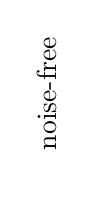
\begin{tikzpicture}
            \node[rotate=90] at (0,0) {noise-free};
            \node at (0,-1.) {~};
    \end{tikzpicture}
    & ~&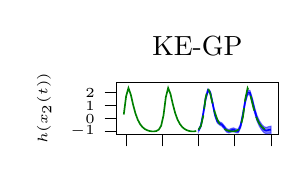
\begin{tikzpicture}
\definecolor{darkgray176}{RGB}{176,176,176}
\definecolor{green}{RGB}{0,128,0}
\definecolor{lightgray204}{RGB}{204,204,204}

\begin{axis}[
    width=.3\textwidth,
    height=.3\textwidth/1.618,
legend cell align={left},
legend style={
  fill opacity=0.8,
  draw opacity=1,
  text opacity=1,
  at={(0.91,0.5)},
  anchor=east,
  draw=lightgray204
},
tick align=outside,
tick pos=left,
title={},
x grid style={darkgray176},
xmin=-1.13387096774194, xmax=1.10161290322581,
yticklabel style = {font = \tiny},
xticklabel style = {font = \tiny},
xtick style={color=black},
y grid style={darkgray176},
ylabel={\tiny $h(x_2(t))$},
ymin=-1.24434151103344, ymax=2.80816290983449,
ytick style={color=black},
title = {KE-GP},
xticklabels={,,}
]
\path [draw=blue, fill=blue, opacity=0.5]
(axis cs:0,-1.02140400442368)
--(axis cs:0,-1.02140400442368)
--(axis cs:0.0322580645161294,-0.652495510938043)
--(axis cs:0.064516129032258,0.262354230312171)
--(axis cs:0.096774193548387,1.38587788384001)
--(axis cs:0.129032258064516,2.07107751409938)
--(axis cs:0.161290322580645,1.91304479941786)
--(axis cs:0.193548387096774,1.096045791632)
--(axis cs:0.225806451612903,0.200357004994826)
--(axis cs:0.258064516129032,-0.326932623751153)
--(axis cs:0.290322580645161,-0.495624209343708)
--(axis cs:0.32258064516129,-0.596688569965196)
--(axis cs:0.354838709677419,-0.808100150089652)
--(axis cs:0.387096774193548,-1.03672170704366)
--(axis cs:0.419354838709678,-1.10878441422885)
--(axis cs:0.451612903225806,-1.03331327373072)
--(axis cs:0.483870967741935,-0.99727272098956)
--(axis cs:0.516129032258065,-1.08882645506894)
--(axis cs:0.548387096774194,-1.10726816024921)
--(axis cs:0.580645161290323,-0.723733555461454)
--(axis cs:0.612903225806452,0.152487838763009)
--(axis cs:0.645161290322581,1.18784215908192)
--(axis cs:0.67741935483871,1.84425611957173)
--(axis cs:0.709677419354839,1.80857170010343)
--(axis cs:0.741935483870968,1.21010470785975)
--(axis cs:0.774193548387097,0.445552659859597)
--(axis cs:0.806451612903226,-0.170389730294337)
--(axis cs:0.838709677419355,-0.582415954342097)
--(axis cs:0.870967741935484,-0.87900913355136)
--(axis cs:0.903225806451613,-1.09089609316336)
--(axis cs:0.935483870967742,-1.16971564012116)
--(axis cs:0.967741935483871,-1.13517934879613)
--(axis cs:1,-1.13540273943964)
--(axis cs:1,-1.13540273943964)
--(axis cs:1,-0.589336779426036)
--(axis cs:0.967741935483871,-0.628004884616578)
--(axis cs:0.935483870967742,-0.685345208139557)
--(axis cs:0.903225806451613,-0.626077562117123)
--(axis cs:0.870967741935484,-0.433322283840301)
--(axis cs:0.838709677419355,-0.154140726890767)
--(axis cs:0.806451612903226,0.241992316668614)
--(axis cs:0.774193548387097,0.840905006264103)
--(axis cs:0.741935483870968,1.58841412615865)
--(axis cs:0.709677419354839,2.17141849752468)
--(axis cs:0.67741935483871,2.19181159353498)
--(axis cs:0.645161290322581,1.52129728516532)
--(axis cs:0.612903225806452,0.472803433036172)
--(axis cs:0.580645161290323,-0.418231775360382)
--(axis cs:0.548387096774194,-0.814981052272685)
--(axis cs:0.516129032258065,-0.805812210943319)
--(axis cs:0.483870967741935,-0.723072183173576)
--(axis cs:0.451612903225806,-0.766537276945688)
--(axis cs:0.419354838709678,-0.846024662513243)
--(axis cs:0.387096774193548,-0.775135242656734)
--(axis cs:0.354838709677419,-0.545246972883508)
--(axis cs:0.32258064516129,-0.337834021537275)
--(axis cs:0.290322580645161,-0.249386944092397)
--(axis cs:0.258064516129032,-0.089932232208076)
--(axis cs:0.225806451612903,0.433451550518775)
--(axis cs:0.193548387096774,1.32119318186608)
--(axis cs:0.161290322580645,2.12897982235537)
--(axis cs:0.129032258064516,2.28022951849028)
--(axis cs:0.096774193548387,1.58874655999785)
--(axis cs:0.064516129032258,0.460734887662643)
--(axis cs:0.0322580645161294,-0.458020404542072)
--(axis cs:0,-0.830871395563078)
--cycle;

\addplot [semithick, blue]
table {%
0 -0.926137699993381
0.0322580645161294 -0.555257957740058
0.064516129032258 0.361544558987407
0.096774193548387 1.48731222191893
0.129032258064516 2.17565351629483
0.161290322580645 2.02101231088661
0.193548387096774 1.20861948674904
0.225806451612903 0.316904277756801
0.258064516129032 -0.208432427979615
0.290322580645161 -0.372505576718053
0.32258064516129 -0.467261295751236
0.354838709677419 -0.67667356148658
0.387096774193548 -0.905928474850199
0.419354838709678 -0.977404538371049
0.451612903225806 -0.899925275338205
0.483870967741935 -0.860172452081568
0.516129032258065 -0.947319333006131
0.548387096774194 -0.961124606260949
0.580645161290323 -0.570982665410918
0.612903225806452 0.312645635899591
0.645161290322581 1.35456972212362
0.67741935483871 2.01803385655336
0.709677419354839 1.98999509881406
0.741935483870968 1.3992594170092
0.774193548387097 0.64322883306185
0.806451612903226 0.0358012931871385
0.838709677419355 -0.368278340616432
0.870967741935484 -0.65616570869583
0.903225806451613 -0.858486827640242
0.935483870967742 -0.92753042413036
0.967741935483871 -0.881592116706355
1 -0.86236975943284
};
\addlegendentry{Prediction}
\addplot [semithick, green]
table {%
-1.03225806451613 0.310677215876974
-1 1.72509317079231
-0.967741935483871 2.35958067123089
-0.935483870967742 1.85373346773129
-0.903225806451613 1.06436987498561
-0.870967741935484 0.39375284056191
-0.838709677419355 -0.0953849947985607
-0.806451612903226 -0.432355212837299
-0.774193548387097 -0.658219795153289
-0.741935483870968 -0.806783922492113
-0.709677419354839 -0.902169203461053
-0.67741935483871 -0.960134910896678
-0.645161290322581 -0.989464930765762
-0.612903225806452 -0.991868128129937
-0.580645161290323 -0.957961550613222
-0.548387096774193 -0.851288713427186
-0.516129032258065 -0.554026202604845
-0.483870967741935 0.243038106393077
-0.451612903225806 1.65036100981229
-0.419354838709677 2.36177948342126
-0.387096774193548 1.89633107767594
-0.354838709677419 1.10719751036095
-0.32258064516129 0.4266122896035
-0.290322580645161 -0.0722737325925517
-0.258064516129032 -0.416693101024244
-0.225806451612903 -0.64782458667783
-0.193548387096774 -0.80001455124028
-0.161290322580645 -0.897905560333097
-0.129032258064516 -0.957683656959815
-0.096774193548387 -0.988507495349605
-0.064516129032258 -0.992535488744642
-0.032258064516129 -0.961254120271588
};
\addlegendentry{Condition}
\addplot [semithick, green, dash pattern=on 5.55pt off 2.4pt]
table {%
0 -0.860613365987377
0.0322580645161294 -0.580085256941532
0.064516129032258 0.177945140645911
0.096774193548387 1.5730115929598
0.129032258064516 2.35986002626562
0.161290322580645 1.93810188327795
0.193548387096774 1.15045548523349
0.225806451612903 0.460068281182399
0.258064516129032 -0.0486707058542165
0.290322580645161 -0.400673957842
0.32258064516129 -0.637181665597286
0.354838709677419 -0.793075190688397
0.387096774193548 -0.893522844289506
0.419354838709678 -0.955142308935798
0.451612903225806 -0.987467578406421
0.483870967741935 -0.993096551558174
0.516129032258065 -0.964343694128448
0.548387096774194 -0.869419253002998
0.580645161290323 -0.604680161786228
0.612903225806452 0.115439309275864
0.645161290322581 1.49344249770474
0.67741935483871 2.3536498063136
0.709677419354839 1.97891203269848
0.741935483870968 1.19411427928786
0.774193548387097 0.494122687936025
0.806451612903226 -0.024568177750323
0.838709677419355 -0.384290661890491
0.870967741935484 -0.626285716196433
0.903225806451613 -0.785962214418609
0.935483870967742 -0.889018792725728
0.967741935483871 -0.952509769733059
1 -0.986345405974012
};
\addlegendentry{Target}
\legend{}
\end{axis}

\end{tikzpicture}

    & 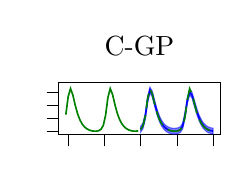
\begin{tikzpicture}
\definecolor{darkgray176}{RGB}{176,176,176}
\definecolor{green}{RGB}{0,128,0}
\definecolor{lightgray204}{RGB}{204,204,204}

\begin{axis}[
    width=.3\textwidth,
    height=.3\textwidth/1.618,
legend cell align={left},
legend style={
  fill opacity=0.8,
  draw opacity=1,
  text opacity=1,
  at={(0.91,0.5)},
  anchor=east,
  draw=lightgray204
},
tick align=outside,
tick pos=left,
title={},
x grid style={darkgray176},
xmin=-1.13387096774194, xmax=1.10161290322581,
yticklabel style = {font = \tiny},
xticklabel style = {font = \tiny},
xtick style={color=black},
y grid style={darkgray176},
yticklabels={,,},
ymin=-1.24434151103344, ymax=2.80816290983449,
ytick style={color=black},
title = {C-GP},
xticklabels={,,}
]
\path [draw=blue, fill=blue, opacity=0.5]
(axis cs:0,-1.05108515937071)
--(axis cs:0,-1.05108515937071)
--(axis cs:0.0322580645161294,-0.793160590795055)
--(axis cs:0.064516129032258,-0.0603062917985711)
--(axis cs:0.096774193548387,1.22882234949531)
--(axis cs:0.129032258064516,1.98426786044561)
--(axis cs:0.161290322580645,1.66841311569064)
--(axis cs:0.193548387096774,0.958310780161869)
--(axis cs:0.225806451612903,0.306394904418292)
--(axis cs:0.258064516129032,-0.212888207688193)
--(axis cs:0.290322580645161,-0.582703101588369)
--(axis cs:0.32258064516129,-0.835874367322634)
--(axis cs:0.354838709677419,-1.00203768354496)
--(axis cs:0.387096774193548,-1.10714748485308)
--(axis cs:0.419354838709678,-1.17140308919753)
--(axis cs:0.451612903225806,-1.19965554864374)
--(axis cs:0.483870967741935,-1.19530653556042)
--(axis cs:0.516129032258065,-1.15936290453452)
--(axis cs:0.548387096774194,-1.0803418364458)
--(axis cs:0.580645161290323,-0.800198044363484)
--(axis cs:0.612903225806452,0.00716944377067719)
--(axis cs:0.645161290322581,1.16755075412088)
--(axis cs:0.67741935483871,1.8172387957578)
--(axis cs:0.709677419354839,1.58508429550798)
--(axis cs:0.741935483870968,0.974585357927645)
--(axis cs:0.774193548387097,0.357310713603246)
--(axis cs:0.806451612903226,-0.15783710235564)
--(axis cs:0.838709677419355,-0.531319888487658)
--(axis cs:0.870967741935484,-0.798065930451727)
--(axis cs:0.903225806451613,-0.97783090509574)
--(axis cs:0.935483870967742,-1.09261986576696)
--(axis cs:0.967741935483871,-1.15862392448967)
--(axis cs:1,-1.18635885172024)
--(axis cs:1,-1.18635885172024)
--(axis cs:1,-0.741559354342373)
--(axis cs:0.967741935483871,-0.713829125691939)
--(axis cs:0.935483870967742,-0.647831583308663)
--(axis cs:0.903225806451613,-0.533053684862027)
--(axis cs:0.870967741935484,-0.353302013267092)
--(axis cs:0.838709677419355,-0.0865646795851854)
--(axis cs:0.806451612903226,0.286913791961969)
--(axis cs:0.774193548387097,0.802061551717969)
--(axis cs:0.741935483870968,1.41933709365362)
--(axis cs:0.709677419354839,2.0298323542427)
--(axis cs:0.67741935483871,2.26198510247366)
--(axis cs:0.645161290322581,1.61229702312937)
--(axis cs:0.612903225806452,0.45191606222082)
--(axis cs:0.580645161290323,-0.355451984459446)
--(axis cs:0.548387096774194,-0.635596974629444)
--(axis cs:0.516129032258065,-0.714619200204716)
--(axis cs:0.483870967741935,-0.750562600662023)
--(axis cs:0.451612903225806,-0.754910083090394)
--(axis cs:0.419354838709678,-0.726655065900912)
--(axis cs:0.387096774193548,-0.662396999060331)
--(axis cs:0.354838709677419,-0.557290313339431)
--(axis cs:0.32258064516129,-0.391130080617812)
--(axis cs:0.290322580645161,-0.137956495689864)
--(axis cs:0.258064516129032,0.231857750074283)
--(axis cs:0.225806451612903,0.751141053470489)
--(axis cs:0.193548387096774,1.40305874079444)
--(axis cs:0.161290322580645,2.11316494792416)
--(axis cs:0.129032258064516,2.4290291703633)
--(axis cs:0.096774193548387,1.6735944055097)
--(axis cs:0.064516129032258,0.384476746922106)
--(axis cs:0.0322580645161294,-0.348367611066797)
--(axis cs:0,-0.606285059749114)
--cycle;

\addplot [semithick, blue]
table {%
0 -0.828685109559914
0.0322580645161294 -0.570764100930926
0.064516129032258 0.162085227561768
0.096774193548387 1.4512083775025
0.129032258064516 2.20664851540445
0.161290322580645 1.8907890318074
0.193548387096774 1.18068476047816
0.225806451612903 0.528767978944391
0.258064516129032 0.00948477119304473
0.290322580645161 -0.360329798639116
0.32258064516129 -0.613502223970223
0.354838709677419 -0.779663998442196
0.387096774193548 -0.884772241956707
0.419354838709678 -0.94902907754922
0.451612903225806 -0.977282815867066
0.483870967741935 -0.972934568111222
0.516129032258065 -0.93699105236962
0.548387096774194 -0.857969405537623
0.580645161290323 -0.577825014411465
0.612903225806452 0.229542752995749
0.645161290322581 1.38992388862513
0.67741935483871 2.03961194911573
0.709677419354839 1.80745832487534
0.741935483870968 1.19696122579063
0.774193548387097 0.579686132660608
0.806451612903226 0.0645383448031647
0.838709677419355 -0.308942284036422
0.870967741935484 -0.57568397185941
0.903225806451613 -0.755442294978883
0.935483870967742 -0.87022572453781
0.967741935483871 -0.936226525090803
1 -0.963959103031306
};
\addlegendentry{Prediction}
\addplot [semithick, green]
table {%
-1.03225806451613 0.303603707030286
-1 1.69110343786114
-0.967741935483871 2.31351669120059
-0.935483870967742 1.81729572009365
-0.903225806451613 1.04295365427054
-0.870967741935484 0.385098409128619
-0.838709677419355 -0.0947311717972172
-0.806451612903226 -0.425288873159369
-0.774193548387097 -0.646855270285042
-0.741935483870968 -0.792592233996031
-0.709677419354839 -0.886162340589994
-0.67741935483871 -0.94302496518416
-0.645161290322581 -0.971796837088032
-0.612903225806452 -0.974154301795878
-0.580645161290323 -0.940892963775511
-0.548387096774193 -0.836250102269154
-0.516129032258065 -0.54464447358633
-0.483870967741935 0.237251764466004
-0.451612903225806 1.61779342401137
-0.419354838709677 2.31567366016837
-0.387096774193548 1.85908270088021
-0.354838709677419 1.08496628312198
-0.32258064516129 0.417332545446167
-0.290322580645161 -0.0720597150884879
-0.258064516129032 -0.409924810099038
-0.225806451612903 -0.636657881807129
-0.193548387096774 -0.785951683345303
-0.161290322580645 -0.881979834254542
-0.129032258064516 -0.940620358416416
-0.096774193548387 -0.970857621592344
-0.064516129032258 -0.974808962590712
-0.032258064516129 -0.944122876092924
};
\addlegendentry{Condition}
\addplot [semithick, green, dash pattern=on 5.55pt off 2.4pt]
table {%
0 -0.845397307426445
0.0322580645161294 -0.570207626173946
0.064516129032258 0.173397512723927
0.096774193548387 1.54191596046199
0.129032258064516 2.31379073013104
0.161290322580645 1.90005861134556
0.193548387096774 1.12740106214391
0.225806451612903 0.450151872143582
0.258064516129032 -0.0489058520877034
0.290322580645161 -0.394210509948319
0.32258064516129 -0.626217494675471
0.354838709677419 -0.779144378277501
0.387096774193548 -0.877680520951649
0.419354838709678 -0.938127372044891
0.451612903225806 -0.969837494186583
0.483870967741935 -0.975359348423147
0.516129032258065 -0.947153655602924
0.548387096774194 -0.854035619106571
0.580645161290323 -0.594334491918945
0.612903225806452 0.112081162395787
0.645161290322581 1.463861058815
0.67741935483871 2.30769869017498
0.709677419354839 1.94009214684081
0.741935483870968 1.17022903279026
0.774193548387097 0.483558226222138
0.806451612903226 -0.0252619931929575
0.838709677419355 -0.378138986826819
0.870967741935484 -0.615528894332488
0.903225806451613 -0.772166761385214
0.935483870967742 -0.873262181133951
0.967741935483871 -0.935544929855583
1 -0.968736676607071
};
\addlegendentry{Target}
\legend{}
\end{axis}

\end{tikzpicture}

    &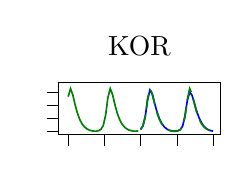
\begin{tikzpicture}
\definecolor{darkgray176}{RGB}{176,176,176}
\definecolor{green}{RGB}{0,128,0}
\definecolor{lightgray204}{RGB}{204,204,204}

\begin{axis}[
    width=.3\textwidth,
    height=.3\textwidth/1.618,
legend cell align={left},
legend style={
  fill opacity=0.8,
  draw opacity=1,
  text opacity=1,
  at={(0.91,0.5)},
  anchor=east,
  draw=lightgray204
},
tick align=outside,
tick pos=left,
title={},
x grid style={darkgray176},
xmin=-1.13387096774194, xmax=1.10161290322581,
yticklabel style = {font = \tiny},
xticklabel style = {font = \tiny},
xtick style={color=black},
y grid style={darkgray176},
ymin=-1.24434151103344, ymax=2.80816290983449,
ytick style={color=black},
yticklabels={,,},
title = {KOR},
xticklabels={,,}
]
\addplot [semithick, blue]
table {%
0 -0.828685109559914
0.0322580645161294 -0.570764100930926
0.064516129032258 0.162085227561768
0.096774193548387 1.4512083775025
0.129032258064516 2.20664851540445
0.161290322580645 1.8907890318074
0.193548387096774 1.18068476047816
0.225806451612903 0.528767978944391
0.258064516129032 0.00948477119304473
0.290322580645161 -0.360329798639116
0.32258064516129 -0.613502223970223
0.354838709677419 -0.779663998442196
0.387096774193548 -0.884772241956707
0.419354838709678 -0.94902907754922
0.451612903225806 -0.977282815867066
0.483870967741935 -0.972934568111222
0.516129032258065 -0.93699105236962
0.548387096774194 -0.857969405537623
0.580645161290323 -0.577825014411465
0.612903225806452 0.229542752995749
0.645161290322581 1.38992388862513
0.67741935483871 2.03961194911573
0.709677419354839 1.80745832487534
0.741935483870968 1.19696122579063
0.774193548387097 0.579686132660608
0.806451612903226 0.0645383448031647
0.838709677419355 -0.308942284036422
0.870967741935484 -0.57568397185941
0.903225806451613 -0.755442294978883
0.935483870967742 -0.87022572453781
0.967741935483871 -0.936226525090803
1 -0.963959103031306
};
\addlegendentry{Prediction}
\addplot [semithick, green]
table {%
-1 1.69110343786114
-0.967741935483871 2.31351669120059
-0.935483870967742 1.81729572009365
-0.903225806451613 1.04295365427054
-0.870967741935484 0.385098409128619
-0.838709677419355 -0.0947311717972172
-0.806451612903226 -0.425288873159369
-0.774193548387097 -0.646855270285042
-0.741935483870968 -0.792592233996031
-0.709677419354839 -0.886162340589994
-0.67741935483871 -0.94302496518416
-0.645161290322581 -0.971796837088032
-0.612903225806452 -0.974154301795878
-0.580645161290323 -0.940892963775511
-0.548387096774193 -0.836250102269154
-0.516129032258065 -0.54464447358633
-0.483870967741935 0.237251764466004
-0.451612903225806 1.61779342401137
-0.419354838709677 2.31567366016837
-0.387096774193548 1.85908270088021
-0.354838709677419 1.08496628312198
-0.32258064516129 0.417332545446167
-0.290322580645161 -0.0720597150884879
-0.258064516129032 -0.409924810099038
-0.225806451612903 -0.636657881807129
-0.193548387096774 -0.785951683345303
-0.161290322580645 -0.881979834254542
-0.129032258064516 -0.940620358416416
-0.096774193548387 -0.970857621592344
-0.064516129032258 -0.974808962590712
-0.032258064516129 -0.944122876092924
};
\addlegendentry{Condition}
\addplot [semithick, green, dash pattern=on 5.55pt off 2.4pt]
table {%
0 -0.845397307426445
0.0322580645161294 -0.570207626173946
0.064516129032258 0.173397512723927
0.096774193548387 1.54191596046199
0.129032258064516 2.31379073013104
0.161290322580645 1.90005861134556
0.193548387096774 1.12740106214391
0.225806451612903 0.450151872143582
0.258064516129032 -0.0489058520877034
0.290322580645161 -0.394210509948319
0.32258064516129 -0.626217494675471
0.354838709677419 -0.779144378277501
0.387096774193548 -0.877680520951649
0.419354838709678 -0.938127372044891
0.451612903225806 -0.969837494186583
0.483870967741935 -0.975359348423147
0.516129032258065 -0.947153655602924
0.548387096774194 -0.854035619106571
0.580645161290323 -0.594334491918945
0.612903225806452 0.112081162395787
0.645161290322581 1.463861058815
0.67741935483871 2.30769869017498
0.709677419354839 1.94009214684081
0.741935483870968 1.17022903279026
0.774193548387097 0.483558226222138
0.806451612903226 -0.0252619931929575
0.838709677419355 -0.378138986826819
0.870967741935484 -0.615528894332488
0.903225806451613 -0.772166761385214
0.935483870967742 -0.873262181133951
0.967741935483871 -0.935544929855583
1 -0.968736676607071
};
\addlegendentry{Target}
\legend{}
\end{axis}

\end{tikzpicture}

    &\definecolor{fig_green}{RGB}{0,128,0}
    \begin{tikzpicture}
        \node at (0,0) {\begin{tikzpicture} 
    \begin{axis}[%
    hide axis,
    xmin=10,
    xmax=50,
    ymin=0,
    ymax=0.4,
    legend style={draw=white!15!black,legend cell align=left}
    ]
    \addlegendimage{semithick, fig_green}
    \addlegendentry{\tiny input};
    \addlegendimage{semithick, fig_green, dash pattern=on 5.55pt off 2.4pt}
    \addlegendentry{\tiny ground truth};
    \addlegendimage{semithick, blue};
    \addlegendentry{\tiny prediction};
    \end{axis}
\end{tikzpicture}};
    \node at (0,-1.) {~};
    \end{tikzpicture}
    \\
    \begin{tikzpicture}
            \node[rotate=90] at (0,0) {noisy};
            \node at (0,-1.65) {~};
    \end{tikzpicture}    
    &~ &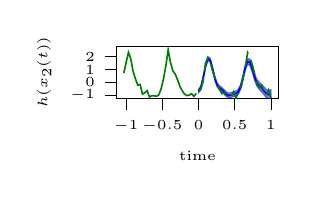
\begin{tikzpicture}
\definecolor{darkgray176}{RGB}{176,176,176}
\definecolor{green}{RGB}{0,128,0}
\definecolor{lightgray204}{RGB}{204,204,204}

\begin{axis}[
    width=.3\textwidth,
    height=.3\textwidth/1.618,
legend cell align={left},
legend style={
  fill opacity=0.8,
  draw opacity=1,
  text opacity=1,
  at={(0.91,0.5)},
  anchor=east,
  draw=lightgray204
},
tick align=outside,
tick pos=left,
title={},
x grid style={darkgray176},
xlabel={\tiny time},
xmin=-1.13387096774194, xmax=1.10161290322581,
yticklabel style = {font = \tiny},
xticklabel style = {font = \tiny},
xtick style={color=black},
y grid style={darkgray176},
ylabel={\tiny $h(x_2(t))$},
ymin=-1.24434151103344, ymax=2.80816290983449,
ytick style={color=black}
]
\path [draw=blue, fill=blue, opacity=0.5]
(axis cs:0,-0.791884136999424)
--(axis cs:0,-0.791884136999424)
--(axis cs:0.0322580645161294,-0.532216532304019)
--(axis cs:0.064516129032258,0.207228559293209)
--(axis cs:0.096774193548387,1.12442474773327)
--(axis cs:0.129032258064516,1.68552099965311)
--(axis cs:0.161290322580645,1.56756057868288)
--(axis cs:0.193548387096774,0.908504125338844)
--(axis cs:0.225806451612903,0.146043870272565)
--(axis cs:0.258064516129032,-0.366882740438619)
--(axis cs:0.290322580645161,-0.596461580106275)
--(axis cs:0.32258064516129,-0.730623805831874)
--(axis cs:0.354838709677419,-0.913165271816812)
--(axis cs:0.387096774193548,-1.10654589884703)
--(axis cs:0.419354838709678,-1.19381854020165)
--(axis cs:0.451612903225806,-1.1546485659785)
--(axis cs:0.483870967741935,-1.08630398785724)
--(axis cs:0.516129032258065,-1.04849802441944)
--(axis cs:0.548387096774194,-0.935844580875931)
--(axis cs:0.580645161290323,-0.556390585828836)
--(axis cs:0.612903225806452,0.13874292125789)
--(axis cs:0.645161290322581,0.915902956607306)
--(axis cs:0.67741935483871,1.38730562268057)
--(axis cs:0.709677419354839,1.31274347655288)
--(axis cs:0.741935483870968,0.790708060720758)
--(axis cs:0.774193548387097,0.158464904288433)
--(axis cs:0.806451612903226,-0.298006792955262)
--(axis cs:0.838709677419355,-0.542627672001628)
--(axis cs:0.870967741935484,-0.721536980353704)
--(axis cs:0.903225806451613,-0.942388520552518)
--(axis cs:0.935483870967742,-1.15803749659711)
--(axis cs:0.967741935483871,-1.26309387894733)
--(axis cs:1,-1.24564270290988)
--(axis cs:1,-1.24564270290988)
--(axis cs:1,-0.553480274017001)
--(axis cs:0.967741935483871,-0.609085413130824)
--(axis cs:0.935483870967742,-0.531751521780701)
--(axis cs:0.903225806451613,-0.338120947030914)
--(axis cs:0.870967741935484,-0.137210070592655)
--(axis cs:0.838709677419355,0.0221297258593717)
--(axis cs:0.806451612903226,0.24789628860997)
--(axis cs:0.774193548387097,0.68638603957788)
--(axis cs:0.741935483870968,1.30113999406795)
--(axis cs:0.709677419354839,1.80656027208635)
--(axis cs:0.67741935483871,1.86440299114285)
--(axis cs:0.645161290322581,1.37557834692631)
--(axis cs:0.612903225806452,0.581761298262494)
--(axis cs:0.580645161290323,-0.128417100507951)
--(axis cs:0.548387096774194,-0.52080342500663)
--(axis cs:0.516129032258065,-0.644678468860948)
--(axis cs:0.483870967741935,-0.693848595375854)
--(axis cs:0.451612903225806,-0.773011108705527)
--(axis cs:0.419354838709678,-0.8207407389894)
--(axis cs:0.387096774193548,-0.740992616247295)
--(axis cs:0.354838709677419,-0.555241944757114)
--(axis cs:0.32258064516129,-0.380263917490026)
--(axis cs:0.290322580645161,-0.253998834224472)
--(axis cs:0.258064516129032,-0.0324742077203883)
--(axis cs:0.225806451612903,0.47322937545827)
--(axis cs:0.193548387096774,1.22944838870588)
--(axis cs:0.161290322580645,1.88216516482222)
--(axis cs:0.129032258064516,1.99311527479243)
--(axis cs:0.096774193548387,1.42551734614703)
--(axis cs:0.064516129032258,0.501904359793165)
--(axis cs:0.0322580645161294,-0.245188439871079)
--(axis cs:0,-0.509073434700109)
--cycle;

\addplot [semithick, blue]
table {%
0 -0.650478785849767
0.0322580645161294 -0.388702486087549
0.064516129032258 0.354566459543187
0.096774193548387 1.27497104694015
0.129032258064516 1.83931813722277
0.161290322580645 1.72486287175255
0.193548387096774 1.06897625702236
0.225806451612903 0.309636622865418
0.258064516129032 -0.199678474079504
0.290322580645161 -0.425230207165373
0.32258064516129 -0.55544386166095
0.354838709677419 -0.734203608286963
0.387096774193548 -0.923769257547163
0.419354838709678 -1.00727963959552
0.451612903225806 -0.963829837342014
0.483870967741935 -0.890076291616549
0.516129032258065 -0.846588246640194
0.548387096774194 -0.728324002941281
0.580645161290323 -0.342403843168393
0.612903225806452 0.360252109760192
0.645161290322581 1.14574065176681
0.67741935483871 1.62585430691171
0.709677419354839 1.55965187431961
0.741935483870968 1.04592402739435
0.774193548387097 0.422425471933156
0.806451612903226 -0.0250552521726459
0.838709677419355 -0.260248973071128
0.870967741935484 -0.42937352547318
0.903225806451613 -0.640254733791716
0.935483870967742 -0.844894509188906
0.967741935483871 -0.936089646039077
1 -0.899561488463438
};
\addlegendentry{Prediction}
\addplot [semithick, green]
table {%
-1.03225806451613 0.729314096916195
-1 1.5430002430531
-0.967741935483871 2.32204403870171
-0.935483870967742 1.831985798904
-0.903225806451613 0.851433703296098
-0.870967741935484 0.279354081877078
-0.838709677419355 -0.210590170919282
-0.806451612903226 -0.154089766822581
-0.774193548387097 -0.89795080770656
-0.741935483870968 -0.788817886111994
-0.709677419354839 -0.631217039088834
-0.67741935483871 -1.11565489128188
-0.645161290322581 -1.0186823441863
-0.612903225806452 -1.02455755343605
-0.580645161290323 -1.06131914172655
-0.548387096774193 -0.952046399419613
-0.516129032258065 -0.466246020590151
-0.483870967741935 0.262503198938305
-0.451612903225806 1.29173786310598
-0.419354838709677 2.51920556711464
-0.387096774193548 1.54711284138206
-0.354838709677419 0.915038117881071
-0.32258064516129 0.656212982887232
-0.290322580645161 0.221915856154588
-0.258064516129032 -0.281944627110773
-0.225806451612903 -0.633593952285014
-0.193548387096774 -0.895240317440411
-0.161290322580645 -1.00560588014814
-0.129032258064516 -0.974031437037782
-0.096774193548387 -0.866150101663904
-0.064516129032258 -1.07102836219983
-0.032258064516129 -0.835479545663183
};
\addlegendentry{Condition}
\addplot [semithick, green, dash pattern=on 5.55pt off 2.4pt]
table {%
0 -0.739654414051487
0.0322580645161294 -0.518329938112951
0.064516129032258 0.116995492630876
0.096774193548387 1.4830385503286
0.129032258064516 1.92918851810535
0.161290322580645 1.60484919087504
0.193548387096774 0.902948829211309
0.225806451612903 0.360083074779615
0.258064516129032 0.038407028127166
0.290322580645161 -0.535312914336627
0.32258064516129 -0.850668308618081
0.354838709677419 -0.773023157271037
0.387096774193548 -1.12963704153207
0.419354838709678 -1.06214760780795
0.451612903225806 -1.04132234674408
0.483870967741935 -0.728286752014149
0.516129032258065 -1.19049036317343
0.548387096774194 -0.786213082699808
0.580645161290323 -0.567579376473479
0.612903225806452 0.335513082155103
0.645161290322581 1.1374733999599
0.67741935483871 2.30787657939374
0.709677419354839 1.96813566944444
0.741935483870968 1.36715134974877
0.774193548387097 0.675192568868016
0.806451612903226 -0.179955450959619
0.838709677419355 -0.372618434067805
0.870967741935484 -0.210140874568701
0.903225806451613 -0.699218180799252
0.935483870967742 -0.996483428586153
0.967741935483871 -0.577931038414108
1 -1.19679478002127
};
\addlegendentry{Target}
\legend{}
\end{axis}

\end{tikzpicture}

    & 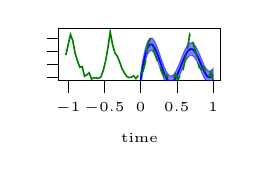
\begin{tikzpicture}
\definecolor{darkgray176}{RGB}{176,176,176}
\definecolor{green}{RGB}{0,128,0}
\definecolor{lightgray204}{RGB}{204,204,204}

\begin{axis}[
    width=.3\textwidth,
    height=.3\textwidth/1.618,
legend cell align={left},
legend style={
  fill opacity=0.8,
  draw opacity=1,
  text opacity=1,
  at={(0.91,0.5)},
  anchor=east,
  draw=lightgray204
},
tick align=outside,
tick pos=left,
title={},
x grid style={darkgray176},
xlabel={\tiny time},
xmin=-1.13387096774194, xmax=1.10161290322581,
yticklabel style = {font = \tiny},
xticklabel style = {font = \tiny},
xtick style={color=black},
y grid style={darkgray176},
ymin=-1.24434151103344, ymax=2.80816290983449,
ytick style={color=black},
yticklabels={,,},
]
\path [draw=blue, fill=blue, opacity=0.5]
(axis cs:0,-1.665446045318)
--(axis cs:0,-1.665446045318)
--(axis cs:0.0322580645161294,-0.568897619418134)
--(axis cs:0.064516129032258,0.263031758801038)
--(axis cs:0.096774193548387,0.80837881476712)
--(axis cs:0.129032258064516,1.06689859178334)
--(axis cs:0.161290322580645,1.05987425552174)
--(axis cs:0.193548387096774,0.827975353710028)
--(axis cs:0.225806451612903,0.427391510412111)
--(axis cs:0.258064516129032,-0.0753940214809364)
--(axis cs:0.290322580645161,-0.609730884208127)
--(axis cs:0.32258064516129,-1.10730328548885)
--(axis cs:0.354838709677419,-1.50844223065865)
--(axis cs:0.387096774193548,-1.76767234362311)
--(axis cs:0.419354838709678,-1.85794397149951)
--(axis cs:0.451612903225806,-1.77307757287024)
--(axis cs:0.483870967741935,-1.52808132186236)
--(axis cs:0.516129032258065,-1.15719445331029)
--(axis cs:0.548387096774194,-0.709747383335965)
--(axis cs:0.580645161290323,-0.244192486820868)
--(axis cs:0.612903225806452,0.179086613560679)
--(axis cs:0.645161290322581,0.505374216416193)
--(axis cs:0.67741935483871,0.692700794731376)
--(axis cs:0.709677419354839,0.717475249796781)
--(axis cs:0.741935483870968,0.577886228992258)
--(axis cs:0.774193548387097,0.294555925632589)
--(axis cs:0.806451612903226,-0.0917064341730509)
--(axis cs:0.838709677419355,-0.52479970843623)
--(axis cs:0.870967741935484,-0.940245125827395)
--(axis cs:0.903225806451613,-1.27320560445854)
--(axis cs:0.935483870967742,-1.46655351593068)
--(axis cs:0.967741935483871,-1.47794982792781)
--(axis cs:1,-1.28506461143995)
--(axis cs:1,-1.28506461143995)
--(axis cs:1,-0.308494704515844)
--(axis cs:0.967741935483871,-0.502960017690905)
--(axis cs:0.935483870967742,-0.491970746399289)
--(axis cs:0.903225806451613,-0.298729000184287)
--(axis cs:0.870967741935484,0.03416669025934)
--(axis cs:0.838709677419355,0.449555573601588)
--(axis cs:0.806451612903226,0.882610046978934)
--(axis cs:0.774193548387097,1.26885004869444)
--(axis cs:0.741935483870968,1.55216499587092)
--(axis cs:0.709677419354839,1.69173937657283)
--(axis cs:0.67741935483871,1.66695089356827)
--(axis cs:0.645161290322581,1.47961336153512)
--(axis cs:0.612903225806452,1.15331907153329)
--(axis cs:0.580645161290323,0.730036686685325)
--(axis cs:0.548387096774194,0.264480380521523)
--(axis cs:0.516129032258065,-0.182967136242761)
--(axis cs:0.483870967741935,-0.553853726218446)
--(axis cs:0.451612903225806,-0.798849088776305)
--(axis cs:0.419354838709678,-0.883714042924335)
--(axis cs:0.387096774193548,-0.79343981256301)
--(axis cs:0.354838709677419,-0.53420442976094)
--(axis cs:0.32258064516129,-0.133056136115851)
--(axis cs:0.290322580645161,0.364529431938274)
--(axis cs:0.258064516129032,0.898881466603521)
--(axis cs:0.225806451612903,1.40168402321776)
--(axis cs:0.193548387096774,1.80229195788188)
--(axis cs:0.161290322580645,2.03423047083746)
--(axis cs:0.129032258064516,2.04131128161313)
--(axis cs:0.096774193548387,1.78285641240048)
--(axis cs:0.064516129032258,1.23761649151677)
--(axis cs:0.0322580645161294,0.406094571417332)
--(axis cs:0,-0.68887762798297)
--cycle;

\addplot [semithick, blue]
table {%
0 -1.17716183665049
0.0322580645161294 -0.0814015240004009
0.064516129032258 0.750324125158903
0.096774193548387 1.2956176135838
0.129032258064516 1.55410493669824
0.161290322580645 1.5470523631796
0.193548387096774 1.31513365579596
0.225806451612903 0.914537766814935
0.258064516129032 0.411743722561292
0.290322580645161 -0.122600726134926
0.32258064516129 -0.620179710802348
0.354838709677419 -1.02132333020979
0.387096774193548 -1.28055607809306
0.419354838709678 -1.37082900721192
0.451612903225806 -1.28596333082327
0.483870967741935 -1.0409675240404
0.516129032258065 -0.670080794776524
0.548387096774194 -0.222633501407221
0.580645161290323 0.242922099932229
0.612903225806452 0.666202842546984
0.645161290322581 0.992493788975658
0.67741935483871 1.17982584414982
0.709677419354839 1.2046073131848
0.741935483870968 1.06502561243159
0.774193548387097 0.781702987163514
0.806451612903226 0.395451806402942
0.838709677419355 -0.0376220674173207
0.870967741935484 -0.453039217784028
0.903225806451613 -0.785967302321414
0.935483870967742 -0.979262131164983
0.967741935483871 -0.990454922809359
1 -0.796779657977895
};
\addlegendentry{Prediction}
\addplot [semithick, green]
table {%
-1.03225806451613 0.729314096916195
-1 1.5430002430531
-0.967741935483871 2.32204403870171
-0.935483870967742 1.831985798904
-0.903225806451613 0.851433703296098
-0.870967741935484 0.279354081877078
-0.838709677419355 -0.210590170919282
-0.806451612903226 -0.154089766822581
-0.774193548387097 -0.89795080770656
-0.741935483870968 -0.788817886111994
-0.709677419354839 -0.631217039088834
-0.67741935483871 -1.11565489128188
-0.645161290322581 -1.0186823441863
-0.612903225806452 -1.02455755343605
-0.580645161290323 -1.06131914172655
-0.548387096774193 -0.952046399419613
-0.516129032258065 -0.466246020590151
-0.483870967741935 0.262503198938305
-0.451612903225806 1.29173786310598
-0.419354838709677 2.51920556711464
-0.387096774193548 1.54711284138206
-0.354838709677419 0.915038117881071
-0.32258064516129 0.656212982887232
-0.290322580645161 0.221915856154588
-0.258064516129032 -0.281944627110773
-0.225806451612903 -0.633593952285014
-0.193548387096774 -0.895240317440411
-0.161290322580645 -1.00560588014814
-0.129032258064516 -0.974031437037782
-0.096774193548387 -0.866150101663904
-0.064516129032258 -1.07102836219983
-0.032258064516129 -0.835479545663183
};
\addlegendentry{Condition}
\addplot [semithick, green, dash pattern=on 5.55pt off 2.4pt]
table {%
0 -0.739654414051487
0.0322580645161294 -0.518329938112951
0.064516129032258 0.116995492630876
0.096774193548387 1.4830385503286
0.129032258064516 1.92918851810535
0.161290322580645 1.60484919087504
0.193548387096774 0.902948829211309
0.225806451612903 0.360083074779615
0.258064516129032 0.038407028127166
0.290322580645161 -0.535312914336627
0.32258064516129 -0.850668308618081
0.354838709677419 -0.773023157271037
0.387096774193548 -1.12963704153207
0.419354838709678 -1.06214760780795
0.451612903225806 -1.04132234674408
0.483870967741935 -0.728286752014149
0.516129032258065 -1.19049036317343
0.548387096774194 -0.786213082699808
0.580645161290323 -0.567579376473479
0.612903225806452 0.335513082155103
0.645161290322581 1.1374733999599
0.67741935483871 2.30787657939374
0.709677419354839 1.96813566944444
0.741935483870968 1.36715134974877
0.774193548387097 0.675192568868016
0.806451612903226 -0.179955450959619
0.838709677419355 -0.372618434067805
0.870967741935484 -0.210140874568701
0.903225806451613 -0.699218180799252
0.935483870967742 -0.996483428586153
0.967741935483871 -0.577931038414108
1 -1.19679478002127
};
\addlegendentry{Target}
\legend{}
\end{axis}

\end{tikzpicture}

    &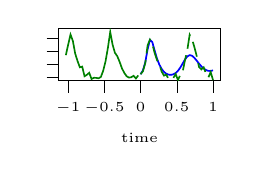
\begin{tikzpicture}
\definecolor{darkgray176}{RGB}{176,176,176}
\definecolor{green}{RGB}{0,128,0}
\definecolor{lightgray204}{RGB}{204,204,204}

\begin{axis}[
    width=.3\textwidth,
    height=.3\textwidth/1.618,
legend cell align={left},
legend style={
  fill opacity=0.8,
  draw opacity=1,
  text opacity=1,
  at={(0.91,0.5)},
  anchor=east,
  draw=lightgray204
},
tick align=outside,
tick pos=left,
title={},
x grid style={darkgray176},
xlabel={\tiny time},
xmin=-1.13387096774194, xmax=1.10161290322581,
yticklabel style = {font = \tiny},
xticklabel style = {font = \tiny},
xtick style={color=black},
y grid style={darkgray176},
ymin=-1.24434151103344, ymax=2.80816290983449,
ytick style={color=black},
yticklabels={,,},
]
\path [draw=blue, fill=blue, opacity=0.5]
(axis cs:0,-0.739898853705199)
--(axis cs:0,-0.739898853705199)
--(axis cs:0.0322580645161294,-0.442945945873865)
--(axis cs:0.064516129032258,0.177347417694429)
--(axis cs:0.096774193548387,1.1793753362096)
--(axis cs:0.129032258064516,1.9082301566808)
--(axis cs:0.161290322580645,1.74112809427527)
--(axis cs:0.193548387096774,1.0935983658069)
--(axis cs:0.225806451612903,0.475966804677645)
--(axis cs:0.258064516129032,0.00745292875602004)
--(axis cs:0.290322580645161,-0.330334796939457)
--(axis cs:0.32258064516129,-0.563439462459379)
--(axis cs:0.354838709677419,-0.705507882191618)
--(axis cs:0.387096774193548,-0.775254931041344)
--(axis cs:0.419354838709678,-0.789205189430896)
--(axis cs:0.451612903225806,-0.750487798384455)
--(axis cs:0.483870967741935,-0.651092336115223)
--(axis cs:0.516129032258065,-0.478710653656521)
--(axis cs:0.548387096774194,-0.227412542331311)
--(axis cs:0.580645161290323,0.083543012528116)
--(axis cs:0.612903225806452,0.395990468795268)
--(axis cs:0.645161290322581,0.630876528174991)
--(axis cs:0.67741935483871,0.730448613899942)
--(axis cs:0.709677419354839,0.685308374337714)
--(axis cs:0.741935483870968,0.528205912488009)
--(axis cs:0.774193548387097,0.309887456428381)
--(axis cs:0.806451612903226,0.0779767485881812)
--(axis cs:0.838709677419355,-0.132959994201391)
--(axis cs:0.870967741935484,-0.302395337257076)
--(axis cs:0.903225806451613,-0.4204759409994)
--(axis cs:0.935483870967742,-0.483716978187525)
--(axis cs:0.967741935483871,-0.491757964036874)
--(axis cs:1,-0.446135940069033)
--(axis cs:1,-0.446135940069033)
--(axis cs:1,-0.446135940069033)
--(axis cs:0.967741935483871,-0.491757964036874)
--(axis cs:0.935483870967742,-0.483716978187525)
--(axis cs:0.903225806451613,-0.4204759409994)
--(axis cs:0.870967741935484,-0.302395337257076)
--(axis cs:0.838709677419355,-0.132959994201391)
--(axis cs:0.806451612903226,0.0779767485881812)
--(axis cs:0.774193548387097,0.309887456428381)
--(axis cs:0.741935483870968,0.528205912488009)
--(axis cs:0.709677419354839,0.685308374337714)
--(axis cs:0.67741935483871,0.730448613899942)
--(axis cs:0.645161290322581,0.630876528174991)
--(axis cs:0.612903225806452,0.395990468795268)
--(axis cs:0.580645161290323,0.083543012528116)
--(axis cs:0.548387096774194,-0.227412542331311)
--(axis cs:0.516129032258065,-0.478710653656521)
--(axis cs:0.483870967741935,-0.651092336115223)
--(axis cs:0.451612903225806,-0.750487798384455)
--(axis cs:0.419354838709678,-0.789205189430896)
--(axis cs:0.387096774193548,-0.775254931041344)
--(axis cs:0.354838709677419,-0.705507882191618)
--(axis cs:0.32258064516129,-0.563439462459379)
--(axis cs:0.290322580645161,-0.330334796939457)
--(axis cs:0.258064516129032,0.00745292875602004)
--(axis cs:0.225806451612903,0.475966804677645)
--(axis cs:0.193548387096774,1.0935983658069)
--(axis cs:0.161290322580645,1.74112809427527)
--(axis cs:0.129032258064516,1.9082301566808)
--(axis cs:0.096774193548387,1.1793753362096)
--(axis cs:0.064516129032258,0.177347417694429)
--(axis cs:0.0322580645161294,-0.442945945873865)
--(axis cs:0,-0.739898853705199)
--cycle;

\addplot [semithick, blue]
table {%
0 -0.739898853705199
0.0322580645161294 -0.442945945873865
0.064516129032258 0.177347417694429
0.096774193548387 1.1793753362096
0.129032258064516 1.9082301566808
0.161290322580645 1.74112809427527
0.193548387096774 1.0935983658069
0.225806451612903 0.475966804677645
0.258064516129032 0.00745292875602004
0.290322580645161 -0.330334796939457
0.32258064516129 -0.563439462459379
0.354838709677419 -0.705507882191618
0.387096774193548 -0.775254931041344
0.419354838709678 -0.789205189430896
0.451612903225806 -0.750487798384455
0.483870967741935 -0.651092336115223
0.516129032258065 -0.478710653656521
0.548387096774194 -0.227412542331311
0.580645161290323 0.083543012528116
0.612903225806452 0.395990468795268
0.645161290322581 0.630876528174991
0.67741935483871 0.730448613899942
0.709677419354839 0.685308374337714
0.741935483870968 0.528205912488009
0.774193548387097 0.309887456428381
0.806451612903226 0.0779767485881812
0.838709677419355 -0.132959994201391
0.870967741935484 -0.302395337257076
0.903225806451613 -0.4204759409994
0.935483870967742 -0.483716978187525
0.967741935483871 -0.491757964036874
1 -0.446135940069033
};
\addlegendentry{Prediction}
\addplot [semithick, green]
table {%
-1.03225806451613 0.729314096916195
-1 1.5430002430531
-0.967741935483871 2.32204403870171
-0.935483870967742 1.831985798904
-0.903225806451613 0.851433703296098
-0.870967741935484 0.279354081877078
-0.838709677419355 -0.210590170919282
-0.806451612903226 -0.154089766822581
-0.774193548387097 -0.89795080770656
-0.741935483870968 -0.788817886111994
-0.709677419354839 -0.631217039088834
-0.67741935483871 -1.11565489128188
-0.645161290322581 -1.0186823441863
-0.612903225806452 -1.02455755343605
-0.580645161290323 -1.06131914172655
-0.548387096774193 -0.952046399419613
-0.516129032258065 -0.466246020590151
-0.483870967741935 0.262503198938305
-0.451612903225806 1.29173786310598
-0.419354838709677 2.51920556711464
-0.387096774193548 1.54711284138206
-0.354838709677419 0.915038117881071
-0.32258064516129 0.656212982887232
-0.290322580645161 0.221915856154588
-0.258064516129032 -0.281944627110773
-0.225806451612903 -0.633593952285014
-0.193548387096774 -0.895240317440411
-0.161290322580645 -1.00560588014814
-0.129032258064516 -0.974031437037782
-0.096774193548387 -0.866150101663904
-0.064516129032258 -1.07102836219983
-0.032258064516129 -0.835479545663183
};
\addlegendentry{Condition}
\addplot [semithick, green, dash pattern=on 5.55pt off 2.4pt]
table {%
0 -0.739654414051487
0.0322580645161294 -0.518329938112951
0.064516129032258 0.116995492630876
0.096774193548387 1.4830385503286
0.129032258064516 1.92918851810535
0.161290322580645 1.60484919087504
0.193548387096774 0.902948829211309
0.225806451612903 0.360083074779615
0.258064516129032 0.038407028127166
0.290322580645161 -0.535312914336627
0.32258064516129 -0.850668308618081
0.354838709677419 -0.773023157271037
0.387096774193548 -1.12963704153207
0.419354838709678 -1.06214760780795
0.451612903225806 -1.04132234674408
0.483870967741935 -0.728286752014149
0.516129032258065 -1.19049036317343
0.548387096774194 -0.786213082699808
0.580645161290323 -0.567579376473479
0.612903225806452 0.335513082155103
0.645161290322581 1.1374733999599
0.67741935483871 2.30787657939374
0.709677419354839 1.96813566944444
0.741935483870968 1.36715134974877
0.774193548387097 0.675192568868016
0.806451612903226 -0.179955450959619
0.838709677419355 -0.372618434067805
0.870967741935484 -0.210140874568701
0.903225806451613 -0.699218180799252
0.935483870967742 -0.996483428586153
0.967741935483871 -0.577931038414108
1 -1.19679478002127
};
\addlegendentry{Target}
\legend{}
\end{axis}

\end{tikzpicture}

    &
    \end{tabular}
    
     \vspace{-0.7\intextsep}
\caption{Multi-step mean and 2-sigma interval of the prediction for predator population from the predator-prey dynamics for our proposed Koopman-equivariant GP (KE-GP), a generic contextual kernel (C-GP), and a Koopman operator regression approach (KOR) for noise-free (top) and noisy (bottom) training data.}
\label{fig:illustrative}
\end{figure*}

\label{section:svigps}
GP model scale poorly with the dataset size, requiring $\BigO(N^3)$ computations and $\BigO(N^2)$ memory during training. To address this, in the following we present a sparse GP approximation that uses a variational inference approach. Our approach closely follows stochastic variational inference with sparse GPs \citep{hensmann2013gaussian,Wilk2018}, with some additional modifications to the selection and optimization of inducing points. As discussed at the end of this section, this choice allows considerable scalability during training \ref{itm:Scale}, and presents desirable properties when used in conjunction with our equivariant covariance function.
\subsection{Variational Inference with Sparse GPs}

	During training, computational complexity stems mainly from the inversion of the data covariance matrix $\Kff$, where $\left[\Kff\right]_{nn'} =  k^{\txt{KE}}_y((t,\vz^{(n)}),(t',\vz^{(n^\prime)})) =: k^{\txt{KE}}_{y(t,t^\prime)}(\vz^{(n)},\vz^{(n^\prime)})$. To address these problems, we resort to variational inference using \emph{inducing variables}  \citep{quinonero2005unifying,hensmann2013gaussian}. %
 We obtain the sparse GP by considering $M \ll N$ inducing observations $\vm$, corresponding to the inducing trajectories $\smash{\{{\vz}^{(m)}:=\bm{x}^{(m)}_{[\tau_s,\tau_e]}\}_{m=1}^M = \mZ}$. Instead of employing the GP prior for the trajectories $\vm$ corresponding to $\mZ$, we place a simpler Gaussian prior $q(\cdot)$ over $\vm$, specified by a mean $\vm$ and covariance $\mS$. By leveraging a variational inference argument \citep{hensmann2013gaussian}, we then obtain the approximate Gaussian process posterior %
 $\GP(\tilde{\mu}(\cdot), \tilde{\sigma}^2(\cdot, \cdot))$ with mean and variance
	\begin{align}
 \begin{split}
	\tilde{\mu}(\cdot) {=} & \Kdu\Kuu\inv\vm,\qquad \\  \tilde{\sigma}^2(\cdot, \cdot) {=}& \kdd - \Kdu\Kuu\inv[\Kuu{ -} \mS]\Kuu\inv\Kud \label{eq:varpost}\,
 \end{split}
	\end{align}
	where $[\Kuu]_{ij} = k^{\txt{KE}}_{y(t,t^\prime)}(\vz^{(i)}, \vz^{(j)})$ %
 and $\smash{\Kud = [k^{\txt{KE}}_{y(t,t^\prime)}(\vz^{(m)}, \cdot)]_{m=1}^M}$. The shape of the posterior can be adjusted by changing the values ${\mZ}$ and output mean $\vm$ and variance $\mS$ of the inducing outputs. Here, we follow an approach similar to \cite{hensmann2013gaussian}, which allows us to minimize by sampling batches of data instead of computing the full gradient, improving memory complexity to $\mathcal{O}(BM+M^2)$. We choose the hyperparameters and inducing points jointly by minimizing the loss
 \begin{align}
 \begin{split}
     \textstyle\sum_{i=1}^{N} &\big( %
 {-}\textstyle \frac{1}{2}\log(2\pi\sigma_{\txt{on}}^{2}) {-}\frac{\sigma_{\txt{on}}^{2}}{2}(y_i-\bm{k}_i^\top \Kuu^{-1} \bm{m})^2 
\\ &{-} \textstyle \frac{1}{2} \sigma_{\txt{on}}^2 \tilde{k}_{i,i} {-} \frac{1}{2} \text{tr} \left( \bm{S} \bm{\Lambda}_i \right) \big)
- \text{KL} \left( q(\bm{u}) \| p(\bm{u}) \right),
\end{split}
 \end{align}
where $\bm{k}_i =[k^{\txt{KE}}_{y(t,t^\prime)}({\vz}^{(m)}, \bm{x}^{(i)}_{[\tau_s,\tau_e]})]_{m=1}^M$, $\Lambda_i =  \Kuu^{-1} \bm{k}_i \bm{k}_i^\top \Kuu^{-1}
$, $\tilde{k}_{i,i} = [\Kff - \Kfu \Kuu^{-1} \Kfu]_{ii}$, and $[\Kfu]_{ij} = k^{\txt{KE}}_{y(t,t^\prime)}(\bm{x}^{(i)}_{[\tau_s,\tau_e]},\vz^{(j)})$. However, unlike \cite{hensmann2013gaussian}, we only optimize inducing trajectories and avoid sampling any time/context-related inducing points, which is due to the structure of the spectral decomposition \eqref{eq:KoopObs}. This allows a significant reduction in training complexity compared, e.g., to the generic contextual kernel $k^{\txt{C}}(\cdot,\cdot):=k^{\txt{SE}}(t,t^\prime)\otimes k^{\txt{SE}}(\bm{x}_{0},\bm{x}^\prime_{0})$, 
where inducing points representing time are also optimized.

Due to the structure of our Koopman-equivariant construction, and the resulting benefits in information gain presented in Section \ref{section:analysisofsamplecomplexity}, our approach is also more robust to a lack of correlation between points, an issue commonly observed in conventional sparse GP approximations \citep{Murray2010,HensmanNIPS2015}. In particular, a lower information gain implies that less inducing points are required than with conventional GPs to accurately represent the full posterior \citep{Burt2019RatesRegression}.%





	
\section{NUMERICAL EXPERIMENTS}\label{sec:NumExp}
To demonstrate the applicability of KE-GPs to realistic data, we perform qualitative and quantitative studies on a set of benchmark examples. As a classical dynamical systems example, we choose the predator-prey model; from the robotics domain, we consider expert demonstrations on the halfcheetah environment from D4RL~\citep{fu2020d4rl} and forecast the first state and action; as a high uncertainty example we choose temperature data from the Monash TSF benchmark \citep{godahewa2021monash} taken at \textit{Oikolab} -- demonstrating the usefulness of building in \eqref{eq:KoopObs} structure as a prior for highly complex weather dynamics. Since these datasets provide a single long trajectory, we split off the last chunk as test data and partition the trajectory into $N$ input-task pairs to comply with our model structure.\looseness=-1

\begin{table}[t!]%
    \caption{Comparable nonparametric frameworks.}
    \label{tab:contributionNonparam}
    \centering
    \footnotesize
    \vspace{-2ex}
    \begin{tabular}{l|ccc}
    \toprule
        Method& \ref{itm:Trac} & \ref{itm:Eff} & \ref{itm:Scale}\\
        \midrule
        C-GP \citep{Li2024STkernel} & ({\color{green!80!black}{\text{\cmark}}})   & \color{red!80!black}{\text{\xmark}} & \color{green!80!black}{\text{\cmark}}\\
        KOR \citep{Kostic2022LearningSpaces} & \color{red!80!black}{\text{\xmark}}  & ({\color{green!80!black}{\text{\cmark}}}) & \color{green!80!black}{\text{\cmark}} \\
        {\text{\textbf{KE-GP} (ours)}} & \color{green!80!black}{\text{\cmark}} & \color{green!80!black}{\text{\cmark}} & \color{green!80!black}{\text{\cmark}} \\
        \bottomrule
    \end{tabular}
\end{table}
\begin{table}[t!]%
    \caption{Simulations on small subsets of the Predator-Prey (PP), D4RL Half-Cheetah (D4RL), and Oikolab Temparature (OT) datasets. We report RMSE in mean and standard deviation for 5 runs. Training data are $N$ past trajectories over a unit-normalized interval, discretized using $H$ equidistant points.}
    \label{tab:smallsim}
    \centering
    \footnotesize
    \vspace{-2ex}
    \begin{tabular}{lc|ccc}
    \toprule
      & $N\times H$& \tbm{KE-GP} & C-GP & KOR\\
   \midrule
    PP&32$\times$32 & 0.28$\pm$0.0& 0.60$\pm$0.0 & \textbf{0.27}$\pm$0.0\\
    D4RL&32$\times$16 & 0.46$\pm$0.0& 0.98$\pm$0.0 & \textbf{0.44}$\pm$0.0\\
    OT&32$\times$16 & \textbf{0.63}$\pm$0.0& 0.68$\pm$0.0 & 0.86$\pm$0.0\\
    
        \bottomrule
    \end{tabular}
\end{table}
\begin{table}[t!]%
    \caption{Simulations on large subsets of the Predator-Prey (PP), D4RL Half-Cheetah (D4RL), and Oikolab Temparature (OL) datasets. Training data are $N$ past trajectories over a unit-normalized interval, discretized using $H$ equidistant points.}
    \label{tab:largesim}
    \centering
    \footnotesize
    \vspace{-2ex}
    \begin{tabular}{lc|ccc}
    \toprule
      & $N\times H$& \tbm{KE-GP} & C-GP & KOR\\
   \midrule
    PP &\phantom{0}512$\times$32& \textbf{0.26}$\pm$0.0\phantom{0}& 0.42$\pm$0.0\phantom{0} & 0.53$\pm$0.0\\
    D4RL$\!\!\!$ &3000$\times$16& 0.48$\pm$0.02 & 0.66$\pm$0.07& \textbf{0.44}$\pm$0.0\\
    OT &4000$\times$16& \textbf{0.54}$\pm$0.03& 0.60$\pm$0.02 & 0.71$\pm$0.0\\
    
        \bottomrule
    \end{tabular}
\end{table}
    


\textbf{Baselines~~} To put our novel algorithm into perspective, we compare to two standard approaches: Gaussian Processes with the time-dependent context (C-GP) by \cite{Li2024STkernel} and operator regression for dynamical systems (KOR)~\citep{Kostic2022LearningSpaces} from the \hyperlink{https://github.com/Machine-Learning-Dynamical-Systems/kooplearn}{\txt{kooplearn}} package and equip it with SciPy's \citep{2020SciPy-NMeth} \textit{minimize} for hyperparameter tuning. While Koopman-based, their method does not forecast via a decomposable model akin to \eqref{eq:KoopObs}, but requires taking powers of a $D{\times}D$ dense matrix. 
As summarized in Table~\ref{tab:contributionNonparam}, these two methods exhibit some of the important properties discussed in Section \ref{sec:ProbStat}, such that they are valuable baselines.\looseness=-1

\begin{figure}[t]
    \centering
    
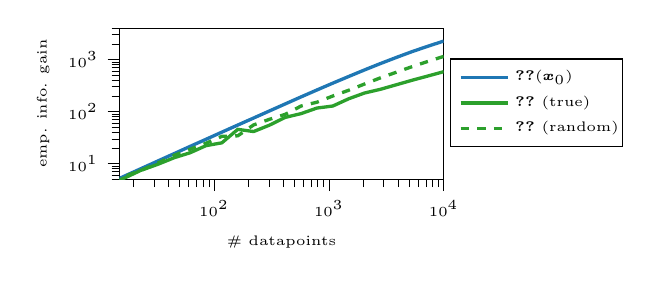
\begin{tikzpicture}

\definecolor{darkgray176}{RGB}{176,176,176}
\definecolor{darkorange25512714}{RGB}{255,127,14}
\definecolor{forestgreen4416044}{RGB}{44,160,44}
\definecolor{lightgray204}{RGB}{204,204,204}
\definecolor{steelblue31119180}{RGB}{31,119,180}



\begin{axis}[
width=5.7cm, height=3.5cm,
legend cell align={left},
legend style={
  at={(1.02,0.8)},
  anchor=north west,
},
tick align=outside,
tick pos=left,
x grid style={darkgray176},
xmin=15, xmax=10000,
xmode=log,
xlabel = {\text{\tiny \# datapoints}},
ylabel = {\text{\tiny emp. info. gain}},
xtick style={color=black},
xtick={0.01,0.1,1,10,100,1000,10000,100000,1000000},
xticklabels={
  \(\displaystyle {10^{-2}}\),
  \(\displaystyle {10^{-1}}\),
  \(\displaystyle {10^{0}}\),
  \(\displaystyle {10^{1}}\),
  \(\displaystyle {10^{2}}\),
  \(\displaystyle {10^{3}}\),
  \(\displaystyle {10^{4}}\),
  \(\displaystyle {10^{5}}\),
  \(\displaystyle {10^{6}}\)
},
y grid style={darkgray176},
ymin=5, ymax=4000,
ymode=log,
ytick style={color=black},
ytick={0.01,0.1,1,10,100,1000,10000,100000},
yticklabels={
  \(\displaystyle {10^{-2}}\),
  \(\displaystyle {10^{-1}}\),
  \(\displaystyle {10^{0}}\),
  \(\displaystyle {10^{1}}\),
  \(\displaystyle {10^{2}}\),
  \(\displaystyle {10^{3}}\),
  \(\displaystyle {10^{4}}\),
  \(\displaystyle {10^{5}}\)
},
yticklabel style = {font = \tiny},
xticklabel style = {font = \tiny},
]
\addplot [very thick, steelblue31119180,]
table {%
9999 2264.11377853996
7278 1804.26327966419
5298 1420.04472403012
3856 1095.40602083438
2807 836.680567640406
2043 631.775979654692
1487 472.562066757352
1082 352.135588183581
788 260.479692402163
573 191.711486161951
417 140.513623368777
303 102.644311381288
221 75.2133200772773
161 55.159666675983
117 40.2831954700074
85 29.31805807427
62 21.4780064745164
45 15.586340006635
32 11.0902089995822
23 7.97107383279624
17 5.89163232362588
12 4.15888308335967
9 3.11916231251975
6 2.07944154167984
4 1.38629436111989
3 1.03972077083992
2 0.693147180559945
1 0.346573590279973
1 0.346573590279973
1 0.346573590279973
};
\addlegendentry{\tiny \ref{eq:SDK}$(\bm{x}_0)$}
\addplot [very thick, forestgreen4416044, ]
table {%
9999 584.656726983284
7278 482.648758569247
5298 400.018580700851
3856 327.016416026596
2807 267.936837961897
2043 227.51171555213
1487 176.282258165846
1082 127.923214142905
788 116.989659625437
573 91.4829039943821
417 77.3576902555283
303 54.7094047705121
221 41.356397075653
161 45.5260312182046
117 25.0994743235434
85 22.1324167310142
62 16.1900860183269
45 12.9863449371233
32 9.59705643999886
23 7.41139449351921
17 5.41375041363105
12 3.95743297067132
9 3.10929738877
6 2.03296155184543
4 1.38344518620096
3 0.987590703724384
2 0.687289146233464
1 0.346573590279973
1 0.346573590279973
1 0.346573590279973
};
\addlegendentry{\tiny \textbf{\ref{eq:KE-SDK}} (true)}

\addplot [very thick, forestgreen4416044, dashed]
table {%
9999 1150.24144167382
7278 921.876964566388
5298 730.129320722141
3856 569.321298285514
2807 444.464772609148
2043 338.563956158658
1487 256.820764550324
1082 199.371251263352
788 151.518582913528
573 128.056611743859
417 88.4672878074439
303 70.909756169937
221 55.4035601061034
161 34.2302972124705
117 33.418917895361
85 24.5881170687663
62 18.9084220075427
45 14.4666214371714
32 10.138627472861
23 7.38739589901983
17 5.79102868865375
12 4.13377361608335
9 3.02188727225571
6 1.93259562627923
4 1.38548323020342
3 1.00804375391702
2 0.69309479616628
1 0.346573590279973
1 0.346573590279973
1 0.346573590279973
};
\addlegendentry{\tiny \textbf{\ref{eq:KE-SDK}} (random)$\!\!\!$}

\end{axis}

\end{tikzpicture}

    \vspace{-1.5\intextsep}
    \caption{Empirical information gain $\hat{\gamma}$ for a 2D linear system scaled to remove effects of constants. %
    The improved rates confirm our theoretical results for Koopman-equivariant GPs, leading to a lower information gain compared to their non-equivariant counterpart \eqref{eq:SDK}, even when a randomly sampled eigenvalue spectrum $\{\eig_j\}_{j=1}^D$  is used instead of the true spectrum.
    }
    \label{fig:enter-label}
\end{figure}
\textbf{Qualitative Comparison~~} We first qualitatively compare the different approaches on the predator-pray model as illustrated in Figure~\ref{fig:illustrative}. It can be clearly seen that all methods allow to accurately predict the future trajectory when given noise-free data from the dynamical system. However, when the state trajectories are perturbed by noise as commonly encountered in practice, significant differences between the predictions become apparent. While our proposed KE-GP maintains a high accuracy and reasonably small confidence intervals, the estimated uncertainty of the C-GP considerably grows and the prediction accuracy for longer horizons significantly drops for the Koopman operator regression (KOR) approach from \cite{Kostic2022LearningSpaces}. This high accuracy of KE-GPs can be attributed to their strong generalization capabilities captured by the information gain as discussed in Section \ref{section:analysisofsamplecomplexity}. When empirically comparing this value, we can immediately see an improvement over non-equivariant kernels, cf. Figure \ref{fig:enter-label}.\looseness=-1

\textbf{Quantitative Evaluation~~} We perform two evaluations for each model run and dataset: a small subset for which exact inference is possible and a large subset handled using variational inference. 
We observe that KE-GP performs robustly on all datasets and sizes as depicted in Tables~\ref{tab:smallsim} and \ref{tab:largesim}. While it consistently outperforms the C-GP, the KOR baseline is better on some datasets but the difference in accuracy is marginal. Importantly, KE-GPs provide a significant improvement over KOR for the other data sets. This is fully in line with our qualitative comparison, which shows that KOR can be sensitive to noise with a severe impact on its performance. In addition, we want to stress here that the KOR method does not come with methods for automated model selection, such that manual parameter tuning was necessary to make it competitive. Therefore, this comparison clearly demonstrates the improved generalization ability achieved by embedding the operator-theoretic foundations in our KE-GP approach.\looseness=-1

    
\section{CONCLUSION}
\label{sec:Concl}
We presented a novel approach to incorporate an operator-theoretic dynamical system structure into Gaussian process regression. Our framework enables a tractable probabilistic treatment of continuous-time dynamical models not present in existing literature. Utilizing a symmetrization tailored to dynamical systems, based on the concept of Koopman-equivariance (KE), we achieve a sample-complexity reduction compared to a contextual kernel without our proposed \eqref{eq:KoopObs} structure. In scaling to large datasets we exploit our model structure to avoid sampling any time/context-related inducing points. Hence, it does not suffer from a lack of correlation between inducing points, which is common for conventional sparse GP.
Through numerical experiments, we show the utility of our KE-GP, demonstrating superior prediction performance to vanilla contextual GPs and on par or better than Koopman operator learning. 


\subsubsection*{Acknowledgements}
This work is supported by the DAAD programme Konrad Zuse Schools of Excellence in Artificial Intelligence (relAI), sponsored by the German Federal Ministry of Education and Research and by the European Research Council (ERC) Consolidator Grant “Safe data-driven control for human-centric systems (CO-MAN)” under grant agreement number 864686.















\appendix
\section*{Appendix}
\section{Discussion: Scope and Ethics}
\label{appendix:scope}
In this work, we evaluate our method on six core scene-aware tasks: existence, count, position, color, scene, and HOI reasoning. We select these tasks as they represent core aspects of multimodal understanding which are essential for many applications. Meanwhile, we do not extend our evaluation to more complex reasoning tasks, such as numerical calculations or code generation, because SOTA diffusion models like SDXL are not yet capable of handling these tasks effectively. Fine-tuning alone cannot overcome the fundamental limitations of these models in generating images that require symbolic logic or complex reasoning. Additionally, we avoid tasks with ethical concerns, such as generating images of specific individuals (e.g., for celebrity recognition task), to mitigate risks related to privacy and misuse. Our goal was to ensure that our approach focuses on technically feasible and responsible AI applications. Expanding to other tasks will require significant advancements in diffusion model capabilities and careful consideration of ethical implications.

\section{Limitations and Future Work}
While our Multimodal Context Evaluator proves effective in enhancing the fidelity of generated images and maintaining diversity, \method is built using pre-trained diffusion models such as SDXL and MLLMs like LLaVA, it inherently shares the limitations of these foundation models. \method still faces challenges with complex reasoning tasks such as numerical calculations or code generation due to the symbolic logic limitations inherent to SDXL. Additionally, during inference, the MLLM context descriptor occasionally generates incorrect information or ambiguous descriptions initially, which can lead to lower fidelity in the generated images. Figure~\ref{fig:failure} further illustrates these observations.

\method currently focuses on single attributes like count, position, and color as part of the multimodal context. This is because this task alone poses significant challenges to existing methods, which \method effectively addresses. A potential direction for future work is to broaden the applicability of \method to synthesize images with multiple scene attributes in the multimodal context as part of compositional reasoning tasks.


\begin{figure}[!h]
    \centering
    \includegraphics[width=\linewidth]{figures/failures.pdf}
    \caption{Failure cases of \method. (a) Our method fails due to the symbolic logic limitation of existing pre-trained SDXL. (b) Initially incorrect descriptions generated by MLLMs lead to low fidelity of generated images. (c) Context description generated by MLLMs is ambiguous and does not directly relate to the text guidance, the spoon can be both inside or outside the bowl.}
    \label{fig:failure}
\end{figure}

\section{Prompt Templates}
\label{appendix:prompts}
Figure~\ref{fig:prompt_templates}~(a-c) showcases the prompt templates used by \method to fine-tune diffusion models specifically on each task including VQA, HOI Reasoning, and Object-Centric benchmarks. It's worth noting that we designed the prompt such that it provides detailed instruction to MLLMs on which scene attributes to focus. We also evaluate the effectiveness of our designed prompt templates by fine-tuning \method with a generic prompt as illustrated in Figure~\ref{fig:prompt_templates}~(d). Table~\ref{table:prommpt} indicates that without using our designed prompt template, the MLLM is not properly instructed to generate specific context description thus leading to reduced performance after fine-tuning on MME tasks. We believe that when using a generic prompt, MLLM is not able to receive sufficient grounding about the multimodal context leading to information loss on key scene attributes.


\begin{table}[!h]
\centering
\footnotesize
\caption{Effectiveness of the prompt template on fine-tuning \method on MME Perception.}
\resizebox{1\linewidth}{!}{
\begin{tabular}{clcccccccccc}
\toprule
 \textbf{MLLM} & \multirow{2}{*}{\textbf{\method}} & \multicolumn{2}{c}{\textbf{Existence}} & \multicolumn{2}{c}{\textbf{Count}} & \multicolumn{2}{c}{\textbf{Position}} & \multicolumn{2}{c}{\textbf{Color}} & \multicolumn{2}{c}{\textbf{Scene}} \\
 \textbf{Name} & & ACC & ACC+ & ACC & ACC+ & ACC & ACC+ & ACC & ACC+ & ACC & ACC+ \\
 \midrule
 \multirow{3}{*}{\makecell{\textbf{LLaVA }  \\ \textbf{v1.6 7B} \\ \citep{liu2024improved}}}
 &w/ prompt template & \textbf{96.67}  & \textbf{93.33}  & \textbf{83.33}  & \textbf{70.00}  & \textbf{81.67}  & \textbf{66.67} & \textbf{95.00}  & \textbf{93.33}  & \textbf{87.75} & \textbf{74.00} \\
 \cmidrule{2-12}
 & \multirow{2}{*}{w/ generic prompt} & 91.67 & 83.33 & 75.00 & 56.67 & \textbf{81.67} & 63.33 & 91.67 & 83.33 & 87.25 & 73.00 \\
 & & {\scriptsize \color{red}\textbf{$\downarrow$ 5.00}} & {\scriptsize \color{red}\textbf{$\downarrow$ 10.00}} & {\scriptsize \color{red}\textbf{$\downarrow$ 8.33}} & {\scriptsize \color{red}\textbf{$\downarrow$ 13.33}} & - &  {\scriptsize \color{red}\textbf{$\downarrow$ 3.34}} & {\scriptsize \color{red}\textbf{$\downarrow$ 3.33}} & {\scriptsize \color{red}\textbf{$\downarrow$ 10.00}} & {\scriptsize \color{red}\textbf{$\downarrow$ 0.50}} & {\scriptsize \color{red}\textbf{$\downarrow$ 1.00}}\\
 \midrule
 \multirow{3}{*}{\makecell{\textbf{InternVL }  \\ \textbf{2.0 8B}\\ \citep{chen2024internvl}}} 
 &w/ prompt template & \textbf{98.33}  & \textbf{96.67} & \textbf{86.67} & \textbf{73.33}  & \textbf{78.33}  & \textbf{63.33}  & \textbf{98.33}  & \textbf{96.67}  & \textbf{86.25} & \textbf{71.00} \\
 \cmidrule{2-12}
 & \multirow{2}{*}{w/ generic prompt} & 91.67 & 83.33 & 80.00 & 60.00 & 71.67 & 50.00 & 91.67 & 83.33 & 84.50 & 69.00 \\
 & & {\scriptsize \color{red}\textbf{$\downarrow$ 6.66}} &  {\scriptsize \color{red}\textbf{$\downarrow$ 13.34}} & {\scriptsize \color{red}\textbf{$\downarrow$ 6.67}} & {\scriptsize \color{red}\textbf{$\downarrow$ 13.33}} & {\scriptsize \color{red}\textbf{$\downarrow$ 6.66}} & {\scriptsize \color{red}\textbf{$\downarrow$ 13.33}} & {\scriptsize \color{red}\textbf{$\downarrow$ 6.66}} & {\scriptsize \color{red}\textbf{$\downarrow$ 13.34}} & {\scriptsize \color{red}\textbf{$\downarrow$ 1.75}} & {\scriptsize \color{red}\textbf{$\downarrow$ 2.00}}\\
\bottomrule
\end{tabular}
}
\label{table:prommpt}
\end{table}

\begin{figure}[!h]
    \centering
    \includegraphics[width=\linewidth]{figures/prompt_template.pdf}
    \caption{Prompt templates (a-c) used by \method to fine-tune the diffusion model on each task including VQA, HOI Reasoning, and Object Centric benchmarks. The generic prompt (d) is also included to evaluate the effectiveness of prompt template.}
    \label{fig:prompt_templates}
\end{figure}
\section{Inference Pipeline}
\label{appendix:inference}
In the inference pipeline of \method (Figure~\ref{fig:inference}), the text guidance $\mathbf{g}$ includes only the question corresponding to the reference image $\mathbf{x}$. The answer is excluded for fair evaluation. Moreover, we remove Multimodal Context Evaluator, and the generated image $\hat{\mathbf{x}}$ is the final output.
\begin{figure}[!h]
    \centering
    \includegraphics[width=\linewidth]{figures/inference.pdf}
    \caption{Inference pipeline of \method}
    \label{fig:inference}
\end{figure}

\begin{figure}[!h]
    \centering
    \includegraphics[width=\linewidth]{figures/diversity_compact_caption.pdf}
    \vspace{-5mm}
    \caption{Examples of context description from MLLM in the inference pipeline where answers are not included in text guidance.}
    \label{fig:diversity_compact_caption}
\end{figure}



\section{Ablation Study on BLIP-2 QFormer}
Our design choice to leverage BLIP-2 QFormer in \method as the multimodal context evaluator facilitates the formulation of our novel Global Semantic and Fine-grained Consistency Rewards. These rewards enable \method to be effective across all tasks as seen in Table~\ref{table:clip}. On replace with a less powerful multimodal context encoder such as CLIP ViT-G/14, we can only implement the global semantic reward as the cosine similarity between the text features and generated image features. As a result, while the setting can maintain performance on coarse-level tasks such as Scene and Existence, there is a noticeable decline on fine-grained tasks like Count and Position. This demonstrates the effectiveness of our design choices in \method and shows that using less powerful alternatives, without the ability to provide both global and fine-grained alignment, affects the fidelity of generated images.

\begin{figure*}[t]
\centering
\includegraphics[width=15.5cm]{figures/clip_zeroshot.png}\\
\caption{CLIP a) training and b) zero-shot inference framework}
\label{fig:clip} 
\end{figure*}


\section{Additional Evaluation on MME Artwork}

To explore the method's ability to work on tasks involving more nuanced or abstract text guidance beyond factual scene attributes, we evaluate \method on an additional task of MME Artwork. This task focuses on image style attributes that are more nuanced/abstract such as the following question-answer pair -- Question: ``Does this artwork exist in the form of mosaic?'', Answer: ``No''.

Table~\ref{table:artwork_reasoning} summarizes the evaluation. We can observe that \method outperforms all existing methods on both ACC and ACC+, implying its higher effectiveness in generating images with high fidelity (in this case, image style preservation) compared to existing methods. This provides evidence that \method can generalize to tasks involving abstract/nuanced attributes such as image style. Figure~\ref{fig:artwork} further shows qualitative comparison between image generation methods on the MME Artwork task.

\begin{table}[h]
\centering
\caption{Comparison on Artwork benchmark and Visual Reasoning task. \method outperforms SOTA image generation and augmentation techniques.}
\resizebox{\linewidth}{!}{
\begin{tabular}{@{}l@{ }ccccccc@{}}
\toprule
\textbf{Method} & \textbf{Real only} & \textbf{RandAugment} &  \textbf{Image Variation} & \textbf{Image Translation} & \textbf{Textual Inversion} & \textbf{I2T2I SDXL} & \textbf{\method} \\
\midrule
\textbf{Artwork ACC} & 69.50 & 69.25 & 69.00 & 67.00 & 66.75 & 68.00 & \textbf{70.25} \\
\textbf{Artwork ACC+} & 41.00 & 41.00 & 40.00 & 38.00 & 37.50 & 38.00 & \textbf{41.50} \\
\midrule
\textbf{Reasoning ACC} & 69.29 & 67.86 & 69.29 & 69.29 & 67.14 & 72.14 & \textbf{72.86} \\
\textbf{Reasoning ACC+} & 42.86 & 40.00 & 41.40 & 40.00 & 37.14 & 47.14 & \textbf{48.57} \\

\bottomrule
\end{tabular}
}
\label{table:artwork_reasoning}
\end{table}


\begin{figure}[!h]
    \centering
    \includegraphics[width=\linewidth]{figures/artwork.pdf}
    \caption{Qualitative comparison on the Artwork task between image generation method. \method can preserve both diversity and fidelity of the reference image in a more abstract domain.}
    \label{fig:artwork}
\end{figure}


\section{Additional Evaluation on MME Commonsense Reasoning}
We have additionally performed our evaluation to more complex tasks such as Visual Reasoning using the MME Commonsense Reasoning benchmark. Results in Table~\ref{table:artwork_reasoning} highlight \method's ability to generalize effectively across diverse domains and complex reasoning tasks, demonstrating its broader applicability. Figure~\ref{fig:reasoning} further shows qualitative comparison between image generation methods on the MME Commonsense Reasoning task.

\begin{figure}[!h]
    \centering
    \includegraphics[width=\linewidth]{figures/reasoning.pdf}
    \caption{Qualitative comparison on the Commonsense Reasoning task between image generation method. \method can preserve both diversity and fidelity of the reference image in a more abstract domain.}
    \label{fig:reasoning}
\end{figure}
\section{FID Scores}
% \textcolor{blue}{We compute FID scores of traditional augmentation and image generation methods. Table~\ref{table:fid} shows that the data distribution of generated images by RandAugment and Image Translation are closer to the real distribution as these methods only change images minimally. We also want to emphasize that even though the FID metric evaluates the quality of generated images, it can not measure the diversity of generated images. \method with rewards fine-tuning achieves a competitive score. As we showed in the diversity analysis in Table~\ref{table:diversity} in the main paper, \method performs significantly better than these ``minimal change" methods while still achieving a competitive FID score. We believe this is a worldwide trade-off.}

We compute FID scores for \method and the different baselines (traditional augmentation and image generation methods) and tabulate the numbers in Table~\ref{table:fid}. FID is a valuable metric for assessing the quality of generated images and how closely the distribution of generated images matches the real distribution. However, \textit{FID does not account for the diversity among the generated images}, which is a critical aspect of the task our work targets~(i.e., how can we generate high fidelity images, preserving certain scene attributes, while still maintaining high diversity?). We also illustrate the shortcomings of FID for the task in Figure~\ref{fig:fid_diversity} where we compare generated images across methods. We observe that RandAugment and Image Translation achieve lower FID scores than \method~(w/ finetuning) because they compromise on diversity by only minimally changing the input image, allowing their generated image distribution to be much closer to the real distribution. While \method has a higher FID score than RandAugment and Image Translation, Figure~\ref{fig:fid_diversity} shows that it is able to preserve the scene attribute w.r.t.~multimodal context while generating an image that is significantly different from than original input image. Therefore, it accomplishes the targeted task more effectively, with both high fidelity and high diversity.

\begin{table}[h]
\centering
\caption{FID scores of traditional augmentation and image generation methods. Lower is better.}
\resizebox{\linewidth}{!}{
\begin{tabular}{@{}l@{ }ccccccc@{}}
\toprule
\multirow{2}{*}{\textbf{Method}} & \multirow{2}{*}{\textbf{RandAugment}} & \multirow{2}{*}{\textbf{I2T2I SDXL}} & \multirow{2}{*}{\textbf{Image Variation}} & \multirow{2}{*}{\textbf{Image Translation}} & \multirow{2}{*}{\textbf{Textual Inversion}} & \multicolumn{2}{c}{\textbf{\method}} \\
& & & & & & \ding{55} fine-tuning & \ding{51} fine-tuning\\
\midrule
\textbf{FID score $\downarrow$} & \textbf{15.93} & 18.35 & 17.66 & 16.29 & 20.84 & 17.78 & 16.55 \\
\bottomrule
\end{tabular}
}
\label{table:fid}
\end{table}

\begin{figure}[!h]
    \centering
    \includegraphics[width=\linewidth]{figures/fid_diversity.pdf}
    \caption{While RandAugment and Image Translation achieve lower FID scores, \method balances fidelity and diversity effectively.}
    \label{fig:fid_diversity}
\end{figure}

\section{User Study}
% \textcolor{blue}{We created a survey form with 50 questions (10 questions per MME task). In each survey question, users were shown: a reference image, a related question, and two generated images from different methods (I2T2I SDXL vs. \method). Users are asked to select the generated image(s) that preserve the attribute referred to by the question in relation to reference image. We collected form responses from 70 people. Table~\ref{table:user_study} shows that \method significantly outperforms I2T2I SDXL in terms of fidelity across all tasks on MME benchmark. We have some examples of survey questions in Figure~\ref{fig:user_study_examples}.}

We conduct a user study where we create a survey form with 50 questions (10 questions per MME Perception task). In each survey question, we show users a reference image, a related question, and a generated image each from two different methods (baseline I2T2I SDXL vs \method). We ask users to select the generated images(s) (either one or both or neither of them) that preserve the attribute referred to by the question in relation to the reference image. If an image is selected, it denotes high fidelity in generation. We collect form responses from 70 people for this study. We compute the percentage of total generated images for each method that were selected by the users as a measure of fidelity. Table~\ref{table:user_study} summarizes the results and shows that \method significantly outperforms I2T2I SDXL in terms of fidelity across all tasks on the MME Perception benchmark. We have some examples of survey questions in Figure~\ref{fig:user_study_examples}.

\begin{figure}[htp]
  \centering
   \includegraphics[width=\columnwidth]{Assets/userstudy_grid.pdf}
   
   \caption{\textbf{User study results.} Users preference percentage of our method compared to other methods in terms of text alignment, visual quality, and overall preference.
   }
   \label{fig:user_study}
\end{figure}
\begin{figure}[!h]
    \centering
    \includegraphics[width=\linewidth]{figures/user_study_examples.pdf}
    \caption{Some examples of our survey questions to evaluate the fidelity of generated images from I2T2I SDXL and \method.}
    \label{fig:user_study_examples}
\end{figure}
\section{Training Performance on Bongard HOI Dataset}
% \textcolor{blue}{We conducted an additional experiment by training a CNN baseline ResNet50 \citep{he2016deep} model on the Bongard-HOI training set with traditional augmentation and other image generation methods, using the same number of training iterations. As shown in Table~\ref{table:hoi_training}, \method consistently outperforms other methods across all test splits. However, as discussed in Subsection~\ref{sec:benchmark_formulation}, our primary focus on test-time evaluation ensures fair comparisons by avoiding variability in training behavior caused by differences in model architectures, data distributions, and training configurations.}

Following the existing method \citep{shu2022testtime}, we conduct an additional experiment by training a ResNet50 \citep{he2016deep} model on the Bongard-HOI \citep{jiang2022bongard} training set with traditional augmentation and Hummingbird generated images. We compare the performance with other image generation methods, using the same
number of training iterations. As shown in Table~\ref{table:hoi_training}, \method consistently outperforms all the baselines across all test splits. In the paper, as discussed in Section~\ref{sec:benchmark_formulation}, we focus primarily on test-time evaluation because it eliminates the variability introduced by model training due to multiple external variables such as model architecture, data distribution, and training configurations, and allows for a fairer comparison where the evaluation setup remains fixed.

\begin{table}[!h]
\centering
\footnotesize
\caption{Comparison on Human-Object Interaction~(HOI) Reasoning by training a CNN-baseline ResNet50 with image augmentation and generation methods. \method outperforms SOTA methods on all $4$ test splits of Bongard-HOI dataset.}
\resizebox{0.8\linewidth}{!}{
\begin{tabular}{lccccc}
\toprule
\multirow{3}{*}{Method} & \multicolumn{4}{c}{Test Splits} & \multirow{3}{*}{Average} \\
\cmidrule{2-5}
 & seen act., & unseen act., & seen act., & unseen act., &  \\
 & seen obj. & seen obj. & unseen obj. & unseen obj. & \\
  % & seen act., seen obj. & unseen act., seen obj. & seen act., unseen obj. & unseen act., unseen obj. &  \\
 % &  &  &  & & \\
\midrule
CNN-baseline (ResNet50) & 50.03\xspace\xspace\xspace\xspace\xspace\xspace\xspace\xspace\xspace\xspace & 49.89\xspace\xspace\xspace\xspace\xspace\xspace\xspace\xspace\xspace\xspace & 49.77\xspace\xspace\xspace\xspace\xspace\xspace\xspace\xspace\xspace\xspace & 50.01\xspace\xspace\xspace\xspace\xspace\xspace\xspace\xspace\xspace\xspace & 49.92\xspace\xspace\xspace\xspace\xspace\xspace\xspace\xspace\xspace\xspace \\
RandAugment \citep{cubuk2020randaugment} & 51.07 {\scriptsize \color{ForestGreen}$\uparrow$ 1.04} & 51.14 {\scriptsize \color{ForestGreen}$\uparrow$ 1.25} & 51.79 {\scriptsize \color{ForestGreen}$\uparrow$ 2.02} & 51.73 {\scriptsize \color{ForestGreen}$\uparrow$ 1.72} & 51.43 {\scriptsize \color{ForestGreen}$\uparrow$ 1.51} \\
Image Variation \citep{xu2023versatile} & 41.78 {\scriptsize \color{red}$\downarrow$ 8.25} & 41.29 {\scriptsize \color{red}$\downarrow$ 8.60} & 41.15 {\scriptsize \color{red}$\downarrow$ 8.62} & 41.25 {\scriptsize \color{red}$\downarrow$ 8.76} & 41.37 {\scriptsize \color{red}$\downarrow$ 8.55} \\
Image Translation \citep{pan2023boomerang} & 46.60 {\scriptsize \color{red}$\downarrow$ 3.43} & 46.94 {\scriptsize \color{red}$\downarrow$ 2.95} & 46.38 {\scriptsize \color{red}$\downarrow$ 3.39} & 46.50 {\scriptsize \color{red}$\downarrow$ 3.51} & 46.61 {\scriptsize \color{red}$\downarrow$ 3.31} \\
Textual Inversion \citep{gal2022image} & \xspace37.67 {\scriptsize \color{red}$\downarrow$ 12.36} & \xspace37.52 {\scriptsize \color{red}$\downarrow$ 12.37} & \xspace38.12 {\scriptsize \color{red}$\downarrow$ 11.65} & \xspace38.06 {\scriptsize \color{red}$\downarrow$ 11.95} & \xspace37.84 {\scriptsize \color{red}$\downarrow$ 12.08} \\
I2T2I SDXL \citep{podell2023sdxl} & 51.92 {\scriptsize \color{ForestGreen}$\uparrow$ 1.89} & 52.18 {\scriptsize \color{ForestGreen}$\uparrow$ 2.29} & 52.25 {\scriptsize \color{ForestGreen}$\uparrow$ 2.48} & 52.15 {\scriptsize \color{ForestGreen}$\uparrow$ 2.14} & 52.13 {\scriptsize \color{ForestGreen}$\uparrow$ 2.21}\\
\textbf{\method} & \textbf{53.71 {\scriptsize \color{ForestGreen}$\uparrow$ 3.68}} & \textbf{53.55 {\scriptsize \color{ForestGreen}$\uparrow$ 3.66}} & \textbf{53.69 {\scriptsize \color{ForestGreen}$\uparrow$ 3.92}} & \textbf{53.41 {\scriptsize \color{ForestGreen}$\uparrow$ 3.40}} & \textbf{53.59 {\scriptsize \color{ForestGreen}$\uparrow$ 3.67}} \\
\bottomrule
\end{tabular}
}
\label{table:hoi_training}
\end{table}



\section{Random Seeds Selection Analysis}
We conduct an additional experiment, varying the number of random seeds from $10$ to $100$. The results are presented in the boxplot in Figure~\ref{fig:boxplot}, which shows the distribution of the mean L2 distances of generated image features from Hummingbird across different numbers of seeds.


The figure demonstrates that the difference in the distribution of the diversity (L2) scores across the different numbers of random seeds is statistically insignificant. So while it is helpful to increase the number of seeds for improved confidence, we observe that it stabilizes at 20 random seeds. This analysis suggests that using $20$ random seeds also suffices to capture the diversity of generated images without significantly affecting the robustness of the analysis.

% We conduct an additional experiment where we vary the number of seeds from 10 to 100. We present the results as a boxplot in Appendix K, Figure 15 which shows the distribution of the mean L2 distances of generated image features from Hummingbird across different numbers of seeds.

% The figure demonstrates that the difference in the distribution of the diversity (L2) scores across the different numbers of random seeds is statistically insignificant. So while it is helpful to increase the number of seeds for improved confidence, we observe that it stabilizes at 20 random seeds. This analysis suggests that using 20 random seeds also suffices to capture the diversity of generated images without significantly affecting the robustness of the analysis.

\begin{figure}[!h]
    \centering
    \includegraphics[width=0.8\linewidth]{figures/diversity_boxplot_rectangular.pdf}
    \caption{Diversity analysis across varying numbers of random seeds (10 to 100) using mean L2 distances of generated image features from \method. The box plot demonstrates consistent diversity scores as the number of seeds increases, indicating that performance stabilizes around 20 random seeds.}
    \label{fig:boxplot}
\end{figure}

\section{Further Explanation of Multimodal Context Evaluator}
The Global Semantic Reward, \(\mathcal{R}_\textrm{global}\), ensures alignment between the global semantic features of the generated image \(\mathbf{\hat{x}}\) and the textual context description \(\mathcal{C}\). This reward leverages cosine similarity to measure the directional alignment between two feature vectors, which can be interpreted as maximizing the mutual information \(I(\mathbf{\hat{x}}, \mathcal{C})\) between the generated image \(\mathbf{\hat{x}}\) and the context description \(\mathcal{C}\). Mutual information quantifies the dependency between the joint distribution \(p_{\theta}(\mathbf{\hat{x}}, \mathcal{C})\) and the marginal distributions. In conditional diffusion models, the likelihood \(p_{\theta}(\mathbf{\hat{x}} \vert \mathcal{C})\) of generating \(\mathbf{\hat{x}}\) given \(\mathcal{C}\) is proportional to the joint distribution:
\[
p_{\theta}(\mathbf{\hat{x}} \vert \mathcal{C}) = \frac{p_{\theta}(\mathbf{\hat{x}}, \mathcal{C})}{p(\mathcal{C})} \propto p_{\theta}(\mathbf{\hat{x}}, \mathcal{C}),
\]
where \(p(\mathcal{C})\) is the marginal probability of the context description, treated as a constant during optimization. By maximizing \(\mathcal{R}_\textrm{global}\), which aligns global semantic features, the model indirectly maximizes the mutual information \(I(\mathbf{\hat{x}}, \mathcal{C})\), thereby enhancing the likelihood \(p_{\theta}(\mathbf{\hat{x}} \vert \mathcal{C})\) in the conditional diffusion model.


The Fine-Grained Consistency Reward, $\mathcal{R}_{\textrm{fine-grained}}$, captures detailed multimodal alignment between the generated image $\mathbf{\hat{x}}$ and the textual context description $\mathcal{C}$. It operates at a token level, leveraging bidirectional self-attention and cross-attention mechanisms in the BLIP-2 QFormer, followed by the Image-Text Matching (ITM) classifier to maximize the alignment score.

\textbf{Self-Attention on Text Tokens:}
    Text tokens $\mathcal{T}_{\mathrm{tokens}}$ undergo self-attention, allowing interactions among words to capture intra-text dependencies:
    \begin{equation}
        \mathcal{T}_{\mathrm{attn}} = \tt{SelfAttention}(\mathcal{T}_{\mathrm{tokens}})
    \end{equation}

\textbf{Self-Attention on Image Tokens:}
    Image tokens $\mathcal{Z}$ are derived from visual features of the generated image $\mathbf{\hat{x}}$ using a cross-attention mechanism:
    \begin{equation}
        \mathcal{Z} = \tt{CrossAttention}(\mathcal{Q}_{\mathrm{learned}}, \mathcal{I}_{\mathrm{tokens}}(\mathbf{\hat{x}}))
    \end{equation}
    These tokens then pass through self-attention to extract intra-image relationships:
    \begin{equation}
        \mathcal{Z}_{\mathrm{attn}} = \tt{SelfAttention}(\mathcal{Z})
    \end{equation}

\textbf{Cross-Attention between Text and Image Tokens:}
    The text tokens $\mathcal{T}_{\mathrm{attn}}$ and image tokens $\mathcal{Z}_{\mathrm{attn}}$ interact through cross-attention to focus on multimodal correlations:
    \begin{equation}
        \mathcal{F} = \tt{CrossAttention}(\mathcal{T}_{\mathrm{attn}}, \mathcal{Z}_{\mathrm{attn}})
    \end{equation}

\textbf{ITM Classifier for Alignment:}
    The resulting multimodal features $\mathcal{F}$ are fed into the ITM classifier, which outputs two logits: one for positive match ($j=1$) and one for negative match ($j=0$). The positive class ($j=1$) indicates strong alignment between the image-text pair, while the negative class ($j=0$) indicates misalignment:
    \begin{equation}
        \mathcal{R}_{\textrm{fine-grained}} = \tt{ITM\_Classifier}(\mathcal{F})_{j=1}
    \end{equation}

The ITM classifier predicts whether the generated image and the textual context description match. Maximizing the logit for the positive class $j=1$ corresponds to maximizing the log probability $\log p(\mathbf{\hat{x}}, \mathcal{C})$ of the joint distribution of image and text. This process aligns the fine-grained details in $\mathbf{\hat{x}}$ with $\mathcal{C}$, increasing the mutual information between the generated image and the text features.

\textbf{Improving fine-grained relationships of CLIP.} While the CLIP Text Encoder, at times, struggles to accurately capture spatial features when processing longer sentences in the Multimodal Context Description, \method addresses this limitation by distilling the global semantic and fine-grained semantic rewards from BLIP-2 QFormer into a specific set of UNet denoiser layers, as mentioned in the implementation details under Appendix~\ref{appendix:impl}~(i.e., Q, V transformation layers including $\tt{to\_q, to\_v, query, value}$). This strengthens the alignment between the generated image tokens~(Q) and input text tokens from the Multimodal Context Description~(K, V) in the cross-attention mechanism of the UNet denoiser. As a result, we obtain generated images with improved fidelity, particularly w.r.t.~spatial relationships, thereby helping to mitigate the shortcomings of vanilla CLIP Text Encoder in processing the long sentences of the Multimodal Context Description.

To illustrate further, a Context Description like “the dog under the pool” is processed in three steps: (1) self-attention is applied to the text tokens (K, V), enabling spatial terms like “dog,” “under,” and “pool” to interact; (2) self-attention is applied to visual features represented by the generated image tokens (Q) to extract intra-image relationships (3) cross-attention aligns this text features with visual features. The resulting alignment scores are used to compute the mean and select the positive class for the reward. Our approach to distill this reward into the cross-attention layers therefore ensures that spatial relationships and other fine-grained attributes are effectively captured, improving the fidelity of generated images.


\section{The Choice of Text Encoder in SDXL and BLIP-2 QFormer}

The choice of text encoder in our pipeline is to leverage pre-trained models for their respective strengths. SDXL inherently uses the CLIP Text Encoder for its generative pipeline, as it is designed to process text embeddings aligned with the CLIP Image Encoder. In the Multimodal Context Evaluator, we use the BLIP-2 QFormer, which is pre-trained with a BERT-based text encoder.

\section{Textual Inversion for Data Augmentation}
In our experiments, we applied Textual Inversion for data augmentation as follows: given a reference image, Textual Inversion learns a new text embedding that captures the context of the reference image (denoted as $<$context$>$). This embedding is then used to generate multiple augmented images by employing the prompt: ``a photo of $<$context$>$". This approach allows Textual Inversion to create context-relevant augmentations for comparison in our experiments.

\section{Convergence Curve}
To evaluate convergence, we monitor the training process using the Global Semantic Reward and Fine-Grained Consistency Reward as criteria. Specifically, we observe the stabilization of these rewards over training iterations. Figure~\ref{fig:convergence} presents the convergence curves for both rewards, illustrating their gradual increase followed by stabilization around 50k iterations. This steady state indicates that the model has learned to effectively align the generated images with the multimodal context.

\begin{figure}[!h]
    \centering
    \includegraphics[width=\linewidth]{figures/convergence.pdf}
    \caption{Convergence curves of Global Semantic and Fine-Grained Consistency Rewards}
    \label{fig:convergence}
\end{figure}


\section{Fidelity Evaluation using GPT-4o}
In addition to the results above, we compute additional metrics for fidelity, which measure how well the model preserves scene attributes when generating new images from a reference image. For this, we use GPT-4o (model version: 2024-05-13) as the MLLM oracle for a VQA task on the MME Perception benchmark \citep{fu2024mme}. 
% We use a MLLM as an oracle for a visual question-answering (VQA) task on the MME Perception benchmark \citep{fu2024mme}. In this experiment, we use GPT-4o (model version: 2024-05-13) as the oracle. 
We evaluate \method with and without fine-tuning process.

The MME dataset consists of Yes/No questions, with a positive and a negative question for every reference image. To measure fidelity, we measure the rate at which the oracle's answer remains consistent across the reference and the generated image for every image in the dataset. We run the experiment multiple times and report the average numbers in Table~\ref{table:fidelity_comparison}. We see that fine-tuning the base SDXL with our novel rewards results in an average increase of $2.99\%$ in fidelity.

\begin{table}[!h]
\centering
\footnotesize
\caption{Fidelity between reference and generated images from \method with and without fine-tuning.}
\resizebox{0.9\linewidth}{!}{
\begin{tabular}{clccc}
\toprule
 \textbf{MLLM Oracle} & \textbf{\method} & \textbf{Fidelity on ``Yes"} & \textbf{Fidelity on ``No"} & \textbf{Overall Fidelity} \\
 \midrule
 \multirow{2}{*}{\makecell{\textbf{GPT-4o}\\\textbf{Ver: 2024-05-13}}}
 & w/o fine-tuning & 68.33\xspace\xspace\xspace\xspace\xspace\xspace\xspace\xspace\xspace\xspace & 70.55\xspace\xspace\xspace\xspace\xspace\xspace\xspace\xspace\xspace\xspace & 71.18\xspace\xspace\xspace\xspace\xspace\xspace\xspace\xspace\xspace\xspace \\
 \cmidrule{2-5}
 % \cmidrule{2-12}
 & w/ fine-tuning & \textbf{69.72} {\scriptsize \color{ForestGreen}\textbf{$\uparrow$ 1.39}}  & \textbf{73.61} {\scriptsize \color{ForestGreen}\textbf{$\uparrow$ 3.06}}  & \textbf{74.17} {\scriptsize \color{ForestGreen}\textbf{$\uparrow$ 2.99}} \\
\bottomrule
\end{tabular}
}
\label{table:fidelity_comparison}
\end{table}


\section{Implementation Details}
\label{appendix:impl}
We implement \method using PyTorch \citep{paszke2019pytorch} and HuggingFace diffusers \citep{huggingface2023diffusers} libraries. For the generative model, we utilize the SDXL Base $1.0$ which is a standard and commonly used pre-trained diffusion model in natural images domain. In the pipeline, we employ CLIP ViT-G/14 as image encoder and both CLIP-L/14 \& CLIP-G/14 as text encoders \citep{radford2021learning}. We perform LoRA fine-tuning on the following modules of SDXL UNet denoiser including $Q$, $V$ transformation layers, fully-connected layers ($\tt{to\_q, to\_v, query, value, ff.net.0.proj}$) with rank parameter $r = 8$, which results in $11$M trainable parameters $\approx 0.46\%$ of total $2.6$B parameters. The fine-tuning is done on $8$ NVIDIA A100 80GB GPUs using AdamW \citep{loshchilov2017decoupled} optimizer, a learning rate of \texttt{5e-6}, and gradient accumulation steps of $8$.

\section{Additional Qualitative Results}
\label{appendix:visuals}
Figure~\ref{fig:diversity_compact_caption} showcases two examples of context description from MLLM in the inference pipeline where answers are not included in text guidance. Figure~\ref{fig:diversity_full} illustrates additional qualitative results highlighting the diversity and multimodal context fidelity between reference and synthetic images, as well as across images generated by \method with different random seeds. Figure~\ref{fig:qualitative_full} shows additional qualitative comparisons between \method and SOTA image generation methods on VQA and HOI Reasoning tasks.
\begin{figure}[!h]
    \centering
    \includegraphics[width=\linewidth]{figures/diversity_full.pdf}
    \vspace{-5mm}
    \caption{Diversity and multimodal context fidelity between reference and synthetic image and across generated ones from \method with different random seeds.}
    \label{fig:diversity_full}
\end{figure}
\begin{figure}[!h]
    \centering
    \includegraphics[width=\linewidth]{figures/qualitative_full_v1.pdf}
    \vspace{-5mm}
    \caption{Qualitative comparison between \method and other image generation methods on MME Perception and HOI Reasoning benchmarks.}
    \label{fig:qualitative_full}
\end{figure}

\end{document}

\typeout{get arXiv to do 4 passes: Label(s) may have changed. Rerun}
